%------------------------------------------------------------------------------
% Plantilla Tesis Maestria
%------------------------------------------------------------------------------

\documentclass[11pt,letterpaper,oneside]{book}
\usepackage[activeacute,spanish]{babel}                                         % Lenguaje de la plantilla.
\usepackage[utf8]{inputenc} 			                                        % Español
\usepackage{ucs}
\usepackage[T1,OT1]{fontenc}                                                    % Fuentes de texto.
%\usepackage{libertine}
\usepackage{latexsym}
\usepackage{amsfonts,amsmath,amssymb}                                           % Simbolo AMS.
\usepackage{graphics,graphicx,rotate,epsfig,color}                              % Grafica.
\usepackage{bibunits}                                                           % Bibliografía.
\usepackage{multirow, array}                                                    % Arreglos y multirenglón.
\usepackage{longtable,multirow,booktabs}
\usepackage[x11names,table]{xcolor}
\usepackage[absolute]{textpos}                                                  % Posición del texto.
\usepackage{pstricks,pst-node,amsopn,subfigure}                                 % Figura flotantes.
\usepackage{IEEEtrantools}                                                      % Herramientas IEEE.
\usepackage{fancyhdr,programs}                                                  % Plantilla fancy y programs.
\usepackage{hhline}                                                             % Separación de columnas.
\usepackage{hyperref}
\usepackage{amsmath,amssymb,amsfonts,latexsym,cancel}
\usepackage{mathtools}
\usepackage{url}
\usepackage{hyperref}
\usepackage{float}
\usepackage[justification=centering]{caption}
\usepackage{graphicx}
\usepackage{float}
\usepackage{algorithm}
%\usepackage{algorithmic}
\usepackage{algpseudocode}
\usepackage{subcaption}
\usepackage{subfigure}
\usepackage{colortbl} % Para colorear celdas de tablas
\usepackage{xcolor}
\spanishdecimal{.}

%%%%%%%%%%%%%%%%%%%%%%%     Nuevos comandos     %%%%%%%%%%%%%%%%%%%%%%%
\newcommand{\mRx}{\mathbf{R}_\mathbf{x}}
\newcommand{\vrx}{\mathbf{r}_\mathbf{x}}
\newcommand{\mathBF}[1]{\mbox{\boldmath $#1$}}
\newcommand{\V}[1]{\mathBF{#1}}
\newcommand{\M}[1]{\mathBF{#1}}

%%%%%%%%%%%%%%%%%%%%%%%     Definición de directorios de trabajo     %%%%%%%%%%%%%%%%%%%%%%%
\newcommand{\DirFigP}{./Figures/Portada}
\newcommand{\DirFigCuno}{./Figures/Capitulo1}
\newcommand{\DirFigCdos}{./Figures/Capitulo2}
\newcommand{\DirFigCtres}{./Figures/Capitulo3}
\newcommand{\DirFigCcuatro}{./Figures/Capitulo4}
\newcommand{\DirFigCcinco}{./Figures/Capitulo5}

%%%%%%%%%%%%%%%%%%%%%%%     Datos personales     %%%%%%%%%%%%%%%%%%%%%%%
\title{\Huge \textsc{Desarrollo de un asistente virtual por reentrenamiento de LLMs con recuperación-generación aumentada desde documentos normativos}}     % Titulo del documento.
\author{\LARGE \textit{Ing. Roberto García Guzmán}}                                                                       % Autor del documento.
\date{Diciembre, 2025}                                                                                                % Fecha de publicación.

%%%%%%%%%%%%%%%%%%%%%%%     Archivos incluidos     %%%%%%%%%%%%%%%%%%%%%%%%%%%%%%%
%  Archivos de tesis
\includeonly{portada}

%  Capítulos
\includeonly{Capitulo1,Capitulo2,Capitulo3,Capitulo4,Conclusiones}
\hyphenation{}

%%%%%%%%%%%%%%%%%%%%%%%     Inicio del documento     %%%%%%%%%%%%%%%%%%%%%%%
\begin{document}

\renewcommand{\tablename}{Tabla}                                                % Cambiar la palabra "Cuadro" por "Tabla"
%\renewcommand{\listtablename}{Índice de Tablas}
\thispagestyle{empty}
\textblockorigin{0mm}{0mm}
\pagestyle{empty}

\begin{textblock}{6}(1.1,1.1)    %1.05, 1.2
    
\includegraphics[width=4.3cm]{\DirFigP/escudo-bn}
\end{textblock}

\begin{textblock}{10}(4.5,1.8)
    \begin{center}
        \huge{UNIVERSIDAD DE GUANAJUATO}
    \end{center}
\end{textblock}

\begin{textblock}{10}(4.8,2.23)
    \begin{flushleft}
        \rule{13cm}{0.5mm}
    \end{flushleft}
\end{textblock}

\begin{textblock}{10}(4.8,2.3)
    \begin{flushleft}
        \rule{13cm}{1.0mm}
    \end{flushleft}
\end{textblock}

\begin{textblock}{10}(4.8,2.4)
    \begin{flushleft}
        \rule{13cm}{0.5mm}
    \end{flushleft}
\end{textblock}

\begin{picture}(0,0)
    \thicklines

    \put(-48,-60){\line(0,-1){530}} \put(-47,-60){\line(0,-1){530}}
    \put(-46,-60){\line(0,-1){530}} \put(-45,-60){\line(0,-1){530}}

    \put(-25,-65){\line(0,-1){535}} \put(-24,-65){\line(0,-1){535}}
    \put(-23,-65){\line(0,-1){535}} \put(-22,-65){\line(0,-1){535}}

    \put(-2,-60){\line(0,-1){530}} \put(-3,-60){\line(0,-1){530}}
    \put(-4,-60){\line(0,-1){530}} \put(-5,-60){\line(0,-1){530}}
\end{picture}

\begin{textblock}{10}(4.5,2.7)
    \begin{center}\Large{CAMPUS IRAPUATO-SALAMANCA\\DIVISIÓN DE INGENIERÍAS}
    \end{center}
\end{textblock}

\begin{textblock}{10}(4.6,4.5)
    \begin{center} \LARGE {\textit{Desarrollo de un asistente virtual por reentrenamiento de LLMs con recuperación-generación aumentada desde documentos normativos}}
    \end{center}
\end{textblock}

\begin{textblock}{12}(3.45,7.0)
    \begin{center} \huge{\bf{TESIS}} \end{center}
\end{textblock}

\begin{textblock}{12}(3.45,8.5)
    \begin{center} \small{\bf{ QUE PARA OBTENER EL TÍTULO DE:}} \end{center}
\end{textblock}

\begin{textblock}{12}(3.45,8.9)
    \begin{center} \emph {MAESTRO EN INGENIERÍA ELÉCTRICA} \end{center}
\end{textblock}

\begin{textblock}{12}(3.6,10.1)
    \begin{center} PRESENTA: \end{center}
\end{textblock}

\begin{textblock}{12}(3.45,10.6)
    \begin{center} \Large{\textit{\textbf{Ing. Roberto García Guzmán}}} \end{center}
\end{textblock}

\begin{textblock}{12}(3.45,12.0)
    \begin{center} DIRECTORES: \end{center}
\end{textblock}

\begin{textblock}{12}(3.45,12.4)
    \begin{center} \large\textit{Dra. Dora Luz Almanza Ojeda}  \end{center}
\end{textblock}

\begin{textblock}{12}(3.45,12.8)
    \begin{center} \large\textit{Dr. Yair Alejandro Andrade Ambriz}  \end{center}
\end{textblock}

\begin{textblock}{9.5}(4.6,14.7)
    \begin{center} SALAMANCA, GTO. \hspace{1.8in} Diciembre, 2025 \end{center}
\end{textblock}

%\begin{textblock}{100}(1.95,4.8)
%\includegraphics[scale=1]{\DirFigP/Porta.eps}
%\end{textblock}

\begin{picture}(0,0)
    \thicklines
\end{picture}

\newpage
                                                      % Portada
\pagestyle{fancy}                                                               % Estilo de página
\fancyhead{}                                                                    % Encabezado de la página
% Aquí se fija el formato de la página
%\paperwidth     =   +8.50in % Ancho del papel
%\paperheight    =   +11.00in% Largo del papel
% Vertical
\voffset        =   +0.00in % Espacio vertical en la página sobre una pulgada

\topmargin      =   -0.40in % Separación entre encabezado y margen
%\headheight     =   +0.25in % Ancho del encabezado
\headheight     =   +0.30in % Ancho del encabezado
%\headsep        =   +0.25in % Separación entre encabezado y cuerpo
\headsep        =   +0.50in % Separación entre encabezado y cuerpo

\textheight     =   +8.00in % Alto del cuerpo

\footskip       =   +0.50in % Suma de separación de cuerpo y ancho de pie

% Horizontal
\hoffset        =   +0.00in % Espacio horizontal en la página sobre una pulgada
%\oddsidemargin  =   +0.50in % Espacio horizontal en páginas par
%\evensidemargin =   +0.25in % Espacio horizontal en página impar
\evensidemargin =   -0.25in % Espacio horizontal en página impar

%\textwidth      =   +4.50in % Ancho del cuerpo
\textwidth      =   +6.00in % Ancho del cuerpo

\marginparsep   =   +0.00in % Separación entre notas y cuerpo
\marginparwidth =   +0.00in % Ancho de notas

\parskip        =   +0.20in % Espacio en encabezado
\lineskip	=   +0.60in
\linespread{1.2}            % Separación entre líneas
\baselineskip  = +0.23in
                                                       % Diseño de hoja
\pagestyle{fancy}       % Estilo de página fancy
\fancyhead{}            % Encabezado de la página
\addtolength{\headwidth}{\marginparsep}
                        % Incrementa la longitud en el encabezado
\addtolength{\headwidth}{\marginparwidth}
                        % Incrementa la longitud en el encabezado
\renewcommand{\headrulewidth}{0.4pt}
                        % Ancho de la regla del encabezado de página
\renewcommand{\footrulewidth}{0.4pt}
                        % Ancho de la regla del pie de página
\renewcommand{\chaptermark}[1]{\markboth {#1}{#1}}
                        % Marca de nombre de capitulo
\renewcommand{\sectionmark}[1]{\markright {\thesection~#1}}
                        % Marca de nombre y numero de sección
%\lhead[\fancyplain{}{\normalsize\scshape\leftmark}]{\fancyplain{}{\small\scshape\rightmark}}
\renewcommand{\baselinestretch}{1.5}

\lhead[\fancyplain{}{\bfseries\thepage}]{\fancyplain{}{\bfseries\rightmark}}
                        % Margen izquierdo superior capitulo o sección
%\rhead[\fancyplain{}{\slshape\leftmark}]{\fancyplain{}{\slshape\rightmark}}
\rhead[\fancyplain{}{\bfseries\leftmark}]{\fancyplain{}{\bfseries}}
                        % Margen derecho superior número de página
%\cfoot{\thepage}
\cfoot{\thepage}                        % Pie de página central
\chead{}
                        % Encabezado de página central

                                                      % Formato de tesis
\pagenumbering{arabic}                                                          % Tipo de letra
%\onehalfspace
%\input{./Chapters/agradecimientos}                                             % Agradecimientos
%\input{./Chapters/institucionales}
\tableofcontents                                                               % Índice general
%\listoffigures

% Índice de figuras
%\listoftables                                                                  % Índice de tablas
%\input{./Chapters/Resumen}		                                                % Prologo
\newpage

%%%%%%%%%%%%%%%%%%%%%%%     Capítulos     %%%%%%%%%%%%%%%%%%%%%%%

%\pagenumbering{arabic}
\chapter{Introducción}

Todas las organizaciones requieren un conjunto de normas para funcionar adecuadamente.
Si bien, en algunas organizaciones, las normas se dan a conocer de forma verbal,
las organizaciones constituidas formalmente requieren que sus lineamientos se encuentren
redactados en documentos para evitar errores o ambigüedades en la
aplicación de los mismos.

En organizaciones grandes, los documentos normativos suelen ser extensos y poseer un
lenguaje que no es familiar para todos los miembros, lo cual puede dificultar el
entendimiento completo de las normas.

Por otro lado, en la última década, se han presentado avances significativos
en lo que popularmente se conoce como \textit{Inteligencia Artificial}, tratándose
específicamente de una mejora notable en los modelos de lenguaje, que ahora
permiten a los sistemas computacionales comunicarse con los usuarios empleando
lenguaje natural y desempeñar tareas relacionadas con la interpretación de texto.

Con el objetivo de aprovechar estas herramientas y favorecer a la comunidad
universitaria, surge el propósito de proveer una herramienta que ayude a conocer
y entender la normativa de la Universidad de Guanajuato. Para ello, se emplearán
técnicas modernas de procesamiento de texto para crear un asistente virtual,
tipo chatbot, que tenga la capacidad de resolver dudas acerca de la los
documentos normativos de la universidad de forma fundamentada, y así, evitar
la vulneración de los derechos de la comunidad y evitar omisiones en el
cumplimiento de sus obligaciones.

\section{Justificación}

La normatividad vigente de la Universidad de Guanajuato (UG) se puede consultar
en su página oficial \footnote{https://www.ugto.mx/}, en la cual se presentan
22 documentos de solo texto en formato PDF que, en conjunto, pesan 6.9 MB. Si
se convierten estos documentos a texto plano, se obtienen 1.1 MB de información,
lo que equivale a 168,011 palabras. Además, la página web presenta otros documentos
relevantes como el Plan de Desarrollo Institucional, la Gaceta Universitaria,
entre otros, los cuales abonan a la cantidad de textos que se espera que
alumnos, docentes y administrativos conozcan y den seguimiento a sus actualizaciones.

Sin embargo, una dificultad que se presenta al momento de divulgar documentos de carácter
oficial es la falta de cultura lectora en la sociedad mexicana. Según
datos del MOLEC 2024 (Módulo de lectura del INEGI) \cite{inegi_modulo_2024},
el porcentaje de población lectora disminuyó 14.6 puntos porcentuales en los últimos
nueve años, pasando del 84.2 \% en 2015 al 69.6 \% en 2024. Aunque se observa
una leve mejora de la cantidad de población lectora con respecto a 2023 (68.5 \%),
la falta de hábitos de lectura en la población es notable. De aquí se
presenta la necesidad de proponer estrategias alternativas en la divulgación de documentos
normativos, como puede ser el uso de asistentes inteligentes.

Por otra parte, el Foro Económico Mundial 2020 (WEF) presentó el concepto de
Educación 4.0 \cite{world_economic_forum_schools_2020}, en la cual se reconoce que la
educación debe adaptarse a las necesidades del futuro y para ello el UNESCO-UNEVOC
(Centro internacional para la Educación y Formación Técnica y Profesional)
define la Educación 4.0 como una técnica de aprendizaje que se centra en
transformar la educación con el uso de tecnologías avanzadas, reconociendo la
Inteligencia Artificial como una de ellas. Alineado con esta visión, este proyecto
pretende servir como ejemplo de la integración de la inteligencia artificial en
el ámbito educativo, para resolver una de las necesidades de la comunidad. Así
mismo, ayudará a fomentar el uso responsable de las tecnologías como los chatbots
inteligentes al emplearlos como herramientas de apoyo en la interpretación de
documentos normativos.

Aunado a lo anterior, desde la introducción de ChatGPT en 2022 \cite{openai_introducing_2022},
los modelos de lenguaje con capacidades conversacionales, o chatbots inteligentes,
se han integraron en diversos ámbitos de la vida cotidiana, siendo el ámbito
académico uno de los más influenciados. Estos cambios motivan a los investigadores
a analizar el impacto que tienen estas herramientas en la educación, como es el
caso de Peláez-Sánchez et al. \cite{pelaez-sanchez_impact_2024}.
Así mismo, se introduce la incógnita de los usos se les puede dar a estas herramientas en
beneficio de la comunidad académica, siendo ésta la motivación del presente proyecto.

Si bien en el mercado actual existen chatbots inteligentes que pueden
responder preguntas relacionadas a documentos que les sean proporcionados, es
difícil proporcionarles todo el contexto necesario para que sus respuestas sean
correctas, que provengan de fuentes autorizadas y estén debidamente
referenciadas. Además, estas herramientas comerciales tienen desventajas
marcadas como que suelen estar sujetas a políticas de uso o privacidad que pueden
ser desfavorables para los usuarios, puede haber variaciones
en su costo, el nivel de personalización es limitado y generalmente se desconoce
el uso que se les da a los datos confidenciales que se comparten en ellas. Lo anterior
obliga a considerar opciones de código abierto, con las que se puede alcanzar
un nivel de personalización mayor, mejor control sobre las políticas de privacidad
y garantizar la continuidad del sistema con un plan adecuado de mantenimiento
y actualización. Es bajo esta filosofía que este proyecto pretende crear un sistema
adaptado a las necesidades de los usuarios y que funcione con opciones de código
abierto.

\section{Antecedentes}

El Procesamiento de Lenguaje Natural (NLP, Natural Language Processing) es una rama
de la inteligencia artificial y la lingüística, dedicada a dotar a las computadoras
de entendimiento de frases o  palabras escritas en lenguajes humanos \cite{khurana_natural_2023}.
En este proyecto, intervienen diferenes áreas del NLP, como son el modelado de lenguaje
(LM, Language Modeling), la respuesta a preguntas (QA, Question Answering) y la
similitud semántica de texto (STS, Semantic Textual Similarity), por mencionar
las más importantes.

Respecto al modelado de lenguaje, es el área del NLP que pretende predecir la siguiente palabra o carácter en una
secuencia de texto dada. En las úlitmas décadas, se han presentado avances significativos
como son: el modelo neuronal probabilístico de Bengio et al. \cite{bengio_neural_2003}
que empleaba una red neuronal y una tabla de búsqueda para predecir el siguiente carácter;
el uso de redes neuronales entrenadas de forma semisupervisada para aprendizaje
multitarea propuesto por Collobert \& Weston \cite{collobert_unified_2008}; la
introducción de embeddings para aprender representaciones vectoriales distribuidas
de las palabras por Mikolov et al. \cite{mikolov_distributed_2013};
la aparición de los modelos sequence-to-sequence que empleaban Memoria a
Largo Corto-Plazo (LSTM) para convertir una secuencia de texto en otra por
Sutskever et al \cite{sutskever_sequence_2014}; la mejora de los modelos
codificador-decodificador empleando mecanismos de atención para detectar partes de la
oración que son relevantes por parte de Bahdanau et al. \cite{bahdanau_neural_2016};
y por último, la introducción de los transformers, los cuales
son una arquitectura de red neuronal basada únicamente en mecanismos de atención
\cite{vaswani_attention_2017} que alcanzaron excelentes resultados en tareas de traducción
máquina. Es en este proceso que surgen los Modelos de Lenguaje de Gran Tamaño
(LLM, Large Language Models), los cuales emplean técnicas de aprendizaje profundo,
particularmente arquitecturas basadas en transformers, para aprender y entender
patrones complejos y estructuras presentes en los datos.

Estos avances llevaron a la creación del Transformer Generativamente Preentrenado
(GPT) por Radford et al. \cite{radford_improving_2018}, una arquitectura basada en
transformers, acompañada de método de entrenamiento que consiste en preentrenar un modelo de
lenguaje para predecir la siguiente palabra, empleando un corpus de texto sin
etiquetar, seguido de un ajuste fino en tareas específicas. Con esta técnica,
fue posible alcanzar resultados superiores al estado del arte en
diversas tareas de NLP, como son la inferencia de lenguaje natural,
dar respuesta a preguntas, búsquedas por similitud semántica, entre otras.

La presentación del modelo GPT fue seguida de mejoras que incluyeron conjuntos de
entrenamiento más extensos, cambios en las técnicas de ajuste fino, incremento en
el tamaño del modelo, entre otras, dando como resultado el lanzamiento de
ChatGPT-3 \cite{openai_introducing_2022}, definido como un modelo que interactúa de forma
conversacional con capacidad de responder preguntas de seguimiento, admitir sus
errores, objetar premisas incorrectas y rechazar peticiones inapropiadas. Tras
la liberación de ChatGPT-3 al público, múltiples empresas y organizaciones han
empleado metodologías de entrenamiento similares para desarrollar sus propios
modelos conversacionales y competir en el mercado.

Estos modelos conversacionales caen en la categoría de chatbots, los cuales se
definen como sistemas computacionales inteligentes con capacidades de conversación,
que son diseñados para emular una conversación humana con el objetivo de
proporcionar orientación o apoyo \cite{caldarini_literature_2022}.

En la actualidad, los modelos generativos basados en transformers como Chat GPT-4
(OpenAI), Gemini (Google), Llama (Meta), DeepSeek (DeepSeek), entre otros, son el
estado del arte en cuanto a chatbots multidominio, ya que pueden responder preguntas
y realizar tareas en diferentes dominios de conocimiento, siendo algunos de ellos
también multimodales. Estos modelos cuentan con varias versiones y tamaños, para
ajustarse a las necesidades de sus usuarios, algunos siendo de paga y otros de
código abierto.

En el ámbito educativo los LLMs han tenido un impacto significativo,
gracias a sus capacidades de generar resúmenes, resaltar partes
importantes de textos, apoyar en tareas de escritura y en general proveer información
a los estudiantes de temas específicos, además de servir a los profesores a generar
material de apoyo personalizado, ayudar en la planeación de las lecciones o para
calificar pruebas de forma semiautomática \cite{kasneci_chatgpt_2023}.

En el ámbito legal se ha explorado el uso de LLMs para apoyar a profesionales
en ley, impuestos y finanzas, como es el caso de la plataforma Harvey.
Esta empresa, a través de una alianza con OpenAI, entrenó un LLM con conocimiento
legal e historial de casos reales, para generar una herramienta tipo chatbot
que puede contestar preguntas teóricas, citar eventos reales y, en general,
funcionar como asistente en la integración y revisión
de casos complejos \cite{openai_customizing_2024}.

En cuanto a las otras áreas del NLP, la presentación del transformer también
derivó en la creación de arquitecturas como BERT (Bidirectional Encoder
Representations from Transformers), presentada por Devlin et al.
\cite{devlin_bert_2019}, la cual tuvo como objetivo generar representaciones
bidireccionales profundas de texto con el objetivo de usarlas en un posterior
proceso de ajuste fino para tareas más específicas, alcanzando resultados
superiores al estado del arte en tareas como la similitud semántica de texto.
Posteriores modificaciones y alternativas a esta arquitectura fueron presentadas
como son el modelo SBERT (Sentence BERT) de Riemers \& Gurevych
\cite{reimers_sentence-bert_2019}, MiniLM de Wang et al \cite{wang_minilm_2020}
o Qwen3 de Zhang et al. \cite{zhang_qwen3_2025} que han demostrado buenos
resultados en tareas de similitud semántica de texto y respuesta a preguntas.

Los modelos mencionados anteriormente hacen uso de diferentes técnicas de ajuste
para obtener los resultados esperados en tareas específicos, de forma general
(y relacionado a este proyecto), las más comunes son: ingeniería de
prompts y el ajuste fino.

La ingeniería de prompts pretende modificar la forma en que un modelo, entrenado
para ello, emita su respuesta a través de instrucciones que se le proporcionan
en forma de texto. Un ejemplo de aplicación de esta técnica se puede ver en el
trabajo de Patil et al. \cite{patil_prompt_2024} que usó instrucciones para
guiar a los modelos a generar explicaciones amigables para los pacientes sobre
conceptos médicos, enfermedades y opciones de tratamiento, con el fin de
reducir la brecha de conocimientos entre médicos y pacientes.

Por otra parte, el ajuste fino es un proceso en el que un modelo preentrenado,
como un LLM, es reentrenado en un conjunto de datos específico para adaptarlo a
tareas o dominios especializados. Dentro de esta metodología existen dos técnicas
ampliamente usadas: Supervised fine-tuning y Reinforcement Learning From Human
Feedback \cite{anisuzzaman_fine-tuning_2025}. Ambas metodologías emplean técnicas
para ajustar el comportamiento del modelo a casos específicos de uso y dotarlo de
comportamientos enfocados en tareas específicas.

Por último, los modelos de lenguaje usualmente enfrentan problemas como las
alucinaciones, la desactualización del conocimiento y la falta de transparencia y
trazabilidad de su proceso de razonamiento. Con el objetivo de aliviar estos
problemas se desarrollaron las técnicas de recuperación-generación aumentada de
información o generación aumentada por recuperación (RAG, Retrieval-Augmented
Generation). Las técnicas RAG consisten en mejorar los LLMs al extraer
fragmentos de información relevante de bases de conocimiento externas, a través
de cálculos de similitud semántica.
Por ejemplo, en una investigación realizada en el ámbito de la medicina, se
encontró que el uso de RAGs en conjunto con LLMs puede mejorar hasta un 39.7 \%
la exactitud en las respuestas de preguntas relacionadas a las normas de la
American Academy of Orthopaedic Surgeons (AAOS), para la atención a lesiones
del ligamento cruzado anterior \cite{woo_custom_2025}.

\section{Objetivos}

\subsection{Objetivo General}

Desarrollar un asistente virtual tipo chatbot, alojado en la nube, que responda
preguntas sobre la normativa de la Universidad de Guanajuato, implementando cuatro
flujos de trabajo: extracción de información con RAGs, reentrenamiento de LLMs,
backend y frontend. Los cuatro flujos de trabajo emplearán técnicas y herramientas
de CI/CD y MLOps o DevOps (según sea el caso) para el despliegue continuo y
actualización del sistema.

\subsection{Objetivos específicos}

\begin{itemize}
      \item Implementar un algoritmo de extracción de información de documentos
            normativos de la universidad de Guanajuato basado en técnicas RAG, que
            pueda interactuar con un modelo LLM.
      \item Reentrenar un LLM que se comunique con el algoritmo de extracción de
            información, para que sea capaz de interpretar la normativa de la Universidad
            de Guanajuato y contestar preguntas relacionadas de forma especializada y
            personalizada, proporcionando referencias de dónde se obtiene la información.
      \item Desarrollar una API, empleando FastAPI o una tecnología similar,
            para comunicar una aplicación cliente con el modelo.
      \item Desarrollar una aplicación web tipo chatbot, empleando React o una
            tecnología similar, para que un usuario pueda hacer consultas al modelo a
            través de internet.
      \item Implementar un flujo de trabajo para el algoritmo de extracción de
            información que permita la actualización automática o semisupervisada de
            la nueva normativa.
      \item Implementar un flujo de trabajo, utilizando herramientas de MLOps,
            para el reentrenamiento, actualización y despliegue del LLM de forma automática
            o semisupervisada.
      \item Implementar un flujo de trabajo para la API y uno para la aplicación
            web, que emplee técnicas y herramientas de CI/CD y DevOps para desplegar
            actualizaciones de forma automática o semisupervisada.
\end{itemize}

\section{Hipótesis del trabajo}

Es posible emplear recuperación-generación aumentada de información con información
de un dominio específico y limitado, así como reentrenar un modelo de lenguaje
para que pueda proporcionar información y resolver dudas que sean entendibles
por personas sin conocimiento previo. La información que se emplee puede
actualizarse con documentos recientes y el modelo puede reentrenarse para mejorar
la calidad de las respuestas basándose en la interacción con los usuarios. Además,
esta metodología puede aplicarse con diferentes fuentes de información, siempre
que se ajuste el modelo al ámbito deseado.

%\chapter{Marco teórico}

En este capítulo se presentan, de forma teórica, los conceptos y técnicas
necesarias para el desarrollo de este proyecto. Se comienza por delimitar
la problemática en el marco del NLP, posteriormente se presentan los
modelos de lenguaje y su aplicación a la problemática, así como la
descripción de la técnica de recuperación-generación aumentada que se empleará,
además de conceptos adicionales necesarios para el desarrollo del proyecto,
por último se presentan trabajos relacionados en el área.

\section{Delimitación de la problemática}

El objetivo de este proyecto es desarrollar un asistente virtual tipo chatbot
que responda preguntas de documentos específicos. Si bien, un asistente
virtual inteligente se desempeña en diferentes áreas del NLP, este proyecto
se centra específicamente en el que se conoce como dar respuesta a preguntas
(QA, Question Answering).

En el contexto del NLP, se entiende como QA al desarrollo de sistemas que
permiten a usuarios emplear interfaces de lenguaje natural para realizar
preguntas y recibir respuestas concisas \cite{pereira_systematic_2022}.
Estos sistemas pueden presentarse de diferentes formas, sin embargo,
actualmente son los modelos de lenguaje de gran tamaño (LLMs) los que
predominan en el área y hacen posible la creación de sistemas que responden
a preguntas de forma interactiva (IQA, Interactive Question Answering),
donde el sistema puede entablar conversaciones con el usuario y responder
las preguntas de forma dinámica \cite{biancofiore_interactive_2024}.

Una parte importante del QA es que, generalmente, funciona con ternas de
información: pregunta, contexto, respuesta. La pregunta y la respuesta
son secuencias de texto en lenguaje natural, y el contexto se refiere a
la información que empleará el modelo para contestar la pregunta, usualmente
el contexto también se encuentra en forma de texto, aunque puede tener
otras formas.

Dentro de los sistemas IQA y QA, existen diferentes elementos a evaluar,
sin embargo la evaluación de la respuesta es el parámetro fundamental en la
mayoría de ellos, para ello se emplean datasets especializados que contienen
preguntas, su contexto y las respectivas respuestas, por ejemplo:
TREC (\textbf{T}ext \textbf{RE}trieval \textbf{C}onference)
\cite{noauthor_proceedings_2001}, Yahoo! (YH) \cite{zhou_learning_2016},
WikiQA \cite{yang_wikiqa_2015}, Standford Question Answering Dataset (SQuAD)
\cite{rajpurkar_squad_2016}, entre otras.


\section{Modelos de lenguaje de gran tamaño (LLMs)}

Para entender lo que es un LLM, primero es necesario presentar el concepto
de red neuronal artificial (ANN, Artificial Neural Network).
Una red neuronal artificial es un modelo dividido en capas de
procesamiento, donde cada capa se compone de nodos o neuronas. Cada neurona
recibe entradas ponderadas, les aplica una transformación y devuelve una
salida. En el modelo tradicional de red neuronal, conocido como
\textit{feedforward}, las salidas de cada capa sirven como entrada de la
siguiente, de esta forma la información se propaga
desde la capa de entrada, pasando por una o más capas ocultas hasta llegar
a la capa de salida, donde se obtiene el resultado final de la red.

Múltiples arquitecturas de ANNs han sido creadas con diferentes propósitos,
y a su vez, se han creado mecanismos que funcionan en conjunto con estas
redes para mejorar su desempeño en tareas específicas. En el contexto del
NLP uno de estos mecanismos es la \textit{atención}. Este mecanismo
fue introducido por Bahdanau et al. \cite{bahdanau_neural_2016} en el contexto
de la traducción de textos automática con el propósito de que una red neuronal
pudiera decidir a qué partes de las oraciones prestar atención.
Si bien Bahdanau no empleaba el término \textit{atención}, su propuesta fue
tomada por Vashwani et al. \cite{vaswani_attention_2017} para crear la
arquitectura del \textit{transformer} para crear una arquitectura basada
únicamente en mecanismos de atención la cual se muestra en la figura
\ref{fig:transformer}.

\begin{figure}[]
    \centering
    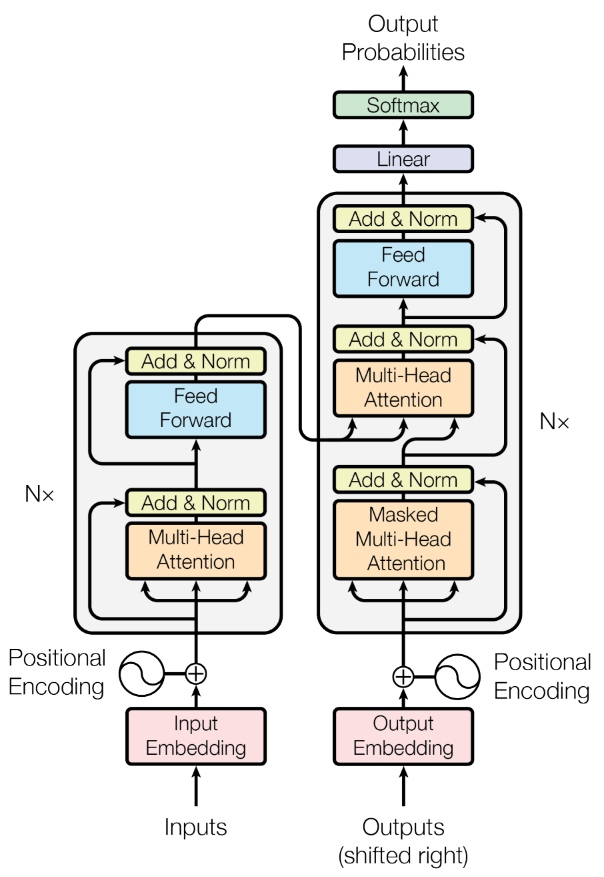
\includegraphics[width = 0.5\textwidth]{\DirFigCdos/transformer}
    \caption{Arquitectura \textit{transformer}. **Cambiar por diagrama en español**}
    \label{fig:transformer}
\end{figure}

El \textit{transformer} esta basado en una arquitectura del tipo
codificador-decodificador, es decir, una red neuronal divida en dos partes
cuyo objetivo es convertir una secuencia de texto a otra.

En su artículo, Vashwani define una función de atención como un mapeo de una
\textit{query} y un conjunto de pares \textit{key}-\textit{value} a una salida,
donde la \textit{query}, las \textit{keys} y los \textit{values} son vectores.
Esta salida es una suma ponderada de los \textit{values}, donde el peso
asignado a cada \textit{value} es calculado por una función de compatibilidad de la
\textit{query} con la \textit{key} correspondiente. Para realizar este
cálculo de forma eficiente se emplea el \textit{Scaled Dot-Product Attention}
definido en la ecuación \ref{eq:attention}.

\begin{equation}\label{eq:attention}
    Attention(Q,K,V) = softmax(\frac{QK^T}{\sqrt{d_k}})V
\end{equation}

Esta operación puede replicarse de forma paralela, con el objetivo de que el
modelo preste atención a información de diferentes representaciones de
subespacios en diferentes posiciones, conformando lo que se denomina
\textit{Multi-Head Attention}, definido por la ecuación \ref{eq:multi_attention}.

\begin{equation}\label{eq:multi_attention}
    \begin{split}
        MultiHead(Q,K,V) = Concat(head_i, ..., head_h)W^O \\
        \text{where } head_i = Attention(QW_i^Q, KW_i^K, VW_i^V)
    \end{split}
\end{equation}

Estos bloques de atención son replicados y combinados en la estructura de
codificador-decodificador, dando como resultado la arquitectura del transformer.
Es de esta arquitectura, que derivan múltiples modelos
con arquitecturas profundas cuyo propósito es realizar tareas relacionadas
con el NLP, a estos modelos se les conoce como LLMs.

\section{\textit{Transformers} pre-entrenados}

Los modelos actuales basados en \textit{transformers} son entrenados de forma
general en dos etapas: Un pre-entrenamiento no supervidado en un corpus
muy grande de texto para hacer modelado de lenguaje estándar, seguido de
un ajuste fino supervisado en tareas específicas empleando datasets
especializados y modificando solamente la salida del modelo. Esta forma de
entrenamiento fue propuesta por Radford et al. \cite{radford_improving_2018},
la cual combinada con el uso de una arquitectura de transformer decodificador
\cite{liu_generating_2018} es la base de los LLM actuales y los empleados en
este proyecto.

\section{Modelos multidominio}

En la actualidad existen LLMs que, además de ser \textit{transformers}
pre-entrenados, pasan por diferentes etapas de ajuste fino, reentrenamiento
en múltiples tareas de diferentes dominios, moderación de respuestas, entre
otras, y además de poseen capacidades conversacionales, como es el caso de
ChatGPT (OpenAI), Gemini (Google), Llama (Meta), entre otros.
Estos modelos, al combinarse con interfaces de usuario amigables y
elementos de aplicaciones comerciales permiten realizar una multitud de
tareas directa o indirectamente relacionadas con NLP, siendo una de ellas
la respuesta a preguntas desde documentos.

Los modelos multidominio, al ser arquitecturas profundas, usualmente se
relacionan con su número de parámetros como métrica de su tamaño, estando
por lo general en el orden de billones. Esta medida es importante pues
sirve para determinar la cantidad aproximada de memoria de video que requieren
para funcionar en su modo de inferencia de acuerdo a la ecuación
\ref{eq:params_to_vram}.

\begin{equation}\label{eq:params_to_vram}
    VRAM(bytes) \approx N_{params} \times \text{bytes-per-param} \times (1 + \alpha)
\end{equation}

\section{Modelos de representaciones vectoriales \textit{embeddings}}

Se llama \textit{embedding} a una representación numérica de una secuencia de
caracteres, que puede ser una palabra o una oración completa. La característica
principal de un \textit{embedding} es que las palabras similares tienen
\textit{embeddings} similares, mientras que palabras u oraciones diferentes u
opuestas tienen \textit{embeddings} muy distintos.

Los modelos con la capacidad de generar representaciones con estas
características se conocen como modelos de \textit{embeddings}. Particularmente,
el modelo SBERT fue creado con este propósito y tiene la característica de
que funciona para oraciones completas de texto, y no solo con palabras.
Otro ejemplo es el modelo Qwen3-Embedding.

\section{Modelos comerciales}

Se entiende por modelos comerciales a aquellos que pertenecen a una entidad
privada y su uso está restringido por el pago de una subscripción.
Además, la arquitectura del modelo, métodos de entrenamiento, así como sus
parámetros de funcionamiento no son públicos. Algunos ejemplos son ChatGPT
(OpenAI), Gemini (Google), Claude (Anthropic), entre otros. Usualmente los
proveedores de estos modelos lo hacen a través de aplicaciones web o APIs,
y en ocasiones, cuentan con versiones gratuitas con capacidades limitadas.

\section{Modelos de código abierto}

Los modelos de código abierto son aquellos que se encuentran disponibles
en sitios especializados, tanto su arquitectura como parámetros de
funcionamiento son accesibles, usualmente a través de una licencia de uso
que usualmente no es restrictiva. Algunos ejemplos son DeepSeek (DeepSeek),
Llama (Meta), Qwen (Qwen), entre otros. Los creadores de estos modelos
generalmente no proveen aplicaciones web o APIs, sino que permiten que los
usuarios o desarrolladores los utilicen en sus propias infraestructuras,
sin depender del creador.

\section{QA con modelos multidominio}

Un modelo multidominio tiene la capacidad de responder preguntas que se
le hagan en lenguaje natural. Para emitir una respuesta lo puede hacer de
diferentes formas.

\subsection{Respuestas desde conocimiento previo}

Durante el entrenamiento del modelo, éste se entrena con corpus de información
muy grande y de diversas fuentes, además de que se le hace un ajuste fino
para esta tarea, de tal forma que el modelo es capaz de responder una pregunta
utilizando la información que se le proporcionó durante su entrenamiento.

Este tipo de respuestas es buena cuando se trata de preguntas de dominio abierto
donde la información es pública y no cambia con el tiempo, como es el caso
de conocimientos generales o eventos históricos.

Sin embargo, las respuestas suelen ser deficientes
cuando se trata de eventos recientes, situaciones personales o conocimiento
restringido, en estos casos se pueden presentar alucinaciones, que son
respuestas cuya estructura es correcta, pero su información es errónea.

Otra limitante es que aunque la respuesta sea correcta, generalmente los
modelos no cuentan con la capacidad de indicar la fuente de la información.

\subsection{Respuestas desde un contexto}

En situaciones donde el modelo no tiene forma de conocer la respuesta porque
no fue entrenado con esa información, es posible proporcionarle un contexto
desde el cual el modelo pueda buscar o inferir la respuesta. Este contexto
usualmente es en forma de texto aunque puede tener otras formas y debe contener
la respuesta. Un ejemplo es proporcionar la información bibliográfica de una
persona como contexto y hacer preguntas sobre la persona o relatar una
situación para hacer una pregunta específica.

Generalmente, estas respuestas son más acertadas, pues los modelos son entrenados
en este tipo de tareas, siempre y cuando el contexto sea adecuado. Una
desventaja de este método es que los modelos operan con ventanas de contexto
limitadas, las cuales pueden ser de algunos miles de tokens hasta unos pocos
millones y es posible que el contexto que se deba proporcionar sea mayor.

\section{Recuperación-Generación Aumentada}

Para superar las limitantes que presentan los LLMs, el uso de técnias de
de Recuperación-Generación Aumentada (RAG, Retrieval-Augmente Generation) ha
sido incorporado con frecuencia. Estas técnicas consisten en incorporar
información o conocimiento desde fuentes de datos externas, que sirven como
complemento a las preguntas \cite{fan_survey_2024}.

Un esquema de RAG simple, como el quese presenta en la figura \ref{fig:rag}
contempla tres etapas principales: Indexado, Recuperación y Generación

\begin{figure}[]
    \centering
    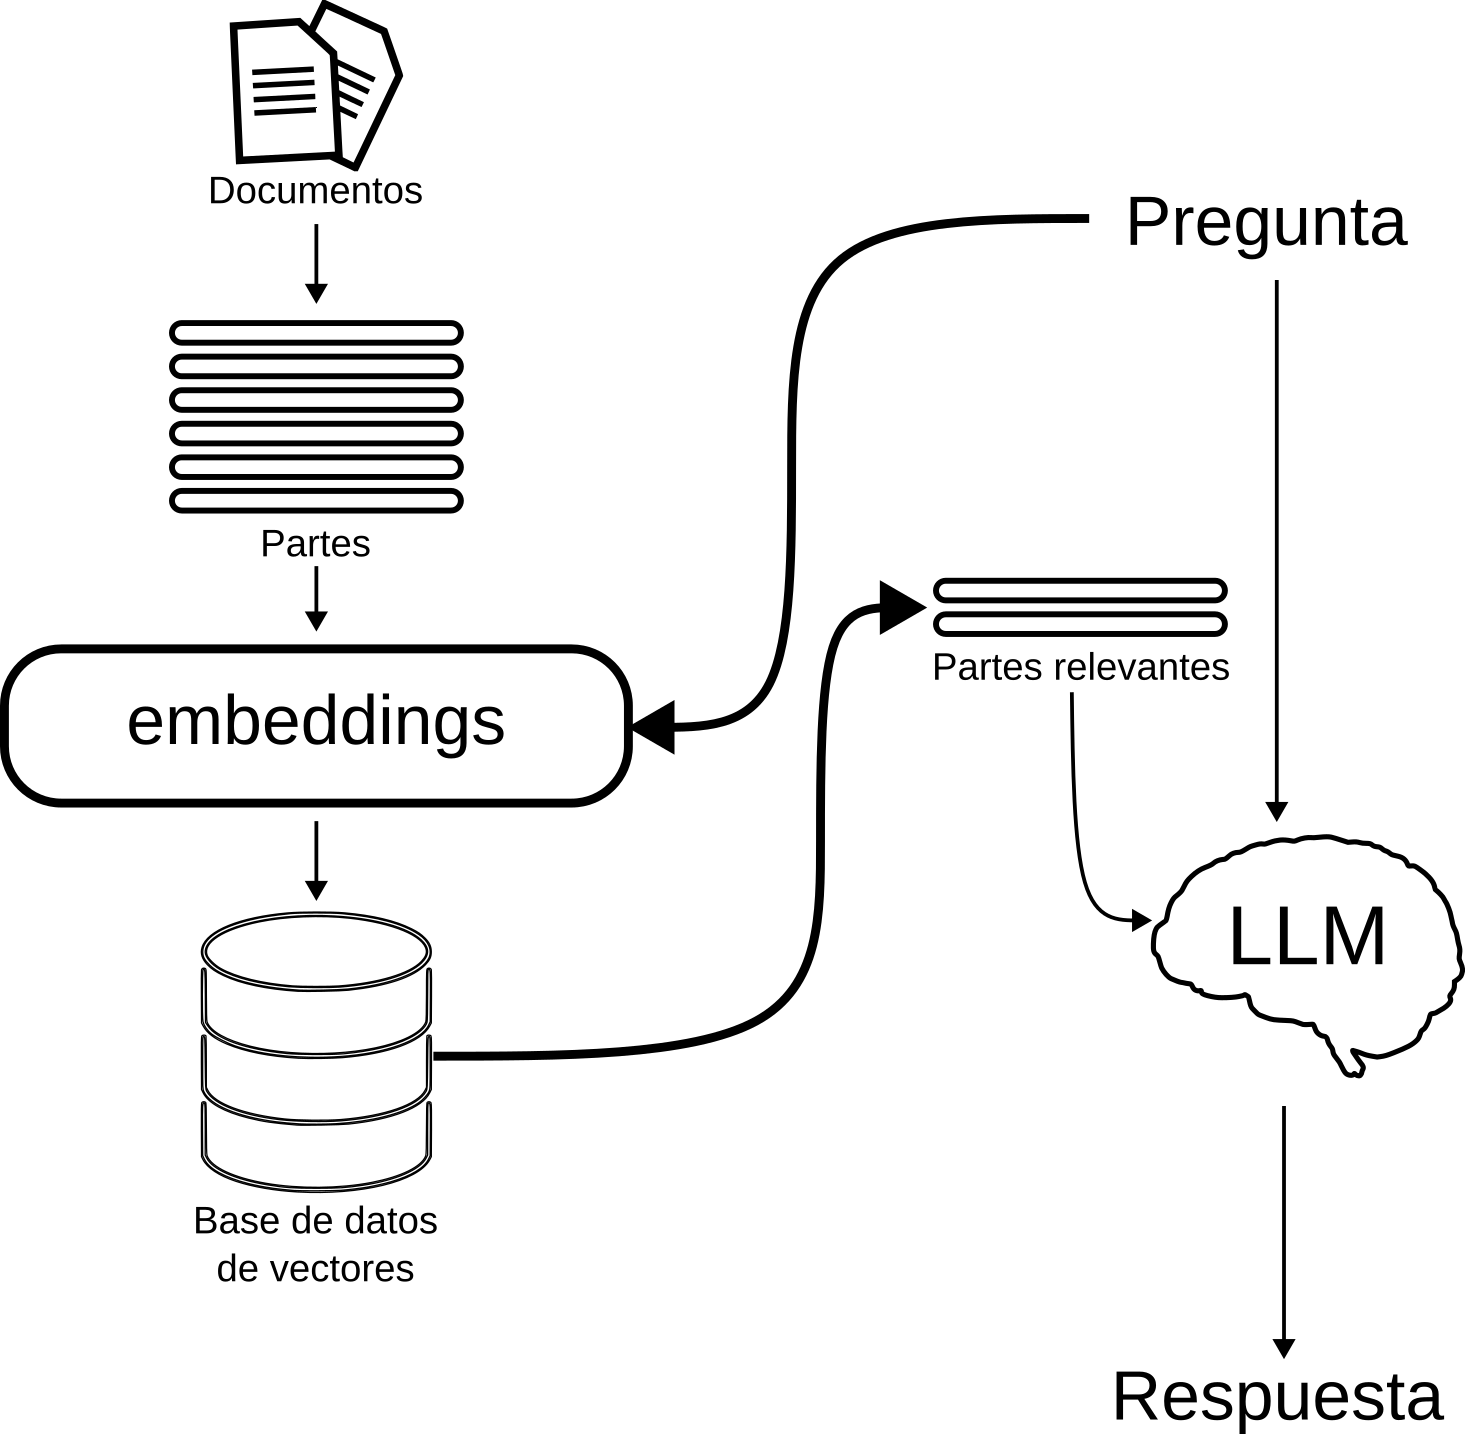
\includegraphics[width = 0.5\textwidth]{\DirFigCdos/simple_rag}
    \caption{Diagrama de funcionamiento de un esquema de RAG simple.}
    \label{fig:rag}
\end{figure}

\subsection{Indexado}

En su forma más simple, una base de conocimiento para RAG parte de la recolección
de documentos relacionados con las preguntas posteriores. Una de las ventajas
es que no hay limitante en la cantidad o tamaño, aunque si deben estar en
formato de texto. Estos documentos se separan en framentos, comunmente
llamados \textit{chunks}, el objetivo es obtener fragmentos pequeños pero
que contengan suficiente información. Posteriormente se calcula la
representación vectoriale (\textit{embedding}) de cada framento, para finalmente
almacenar cada fragmento con su respectivo \textit{embedding} en una base
de datos.

\subsection{Recuperación}

Dada una solicitud hecha al LLM, la recuperación consiste
en buscar información relevante, usualmente en forma de fragmentos de
documentos, en una base de datos previamente construida. La forma de
determinar si un fragmento es relevante o no para la pregunta se mide la
distancia entre la solicitud y el fragmento.

Una de las formas más comunes de medir esta distancia es empleando la
distancia coseno, en su forma de similitud coseno, como se muestra en la
ecuación \ref{eq:cos_similarity}

\begin{equation}\label{eq:cos_similarity}
    d = 1.0 - \frac{\sum{(A_i \times B_i)}}{\sqrt{\sum{(A_i^2)}}\sqrt{\sum{(B_i^2)}}}
\end{equation}

Otra de las métricas comunes es la distancia empleando el producto interno,
como se muestra en la ecuación \ref{eq:inner_product}.

\begin{equation}\label{eq:inner_product}
    d = 1.0 - \sum{(A_i \times B_i)}
\end{equation}

\subsection{Generación}

En esta etapa, tanto la solicitud como los documentos seleccionados son
sintetizados en una instrucción coherente que se le proporciona al modelo.
Usualmente esta instrucción incluye: Indicación de responder la pregunta
solamente con los fragmentos proporcionados, los fragmentos de texto y la
pregunta.

\section{Reentrenamiento de los modelos}

Tanto los LLMs comerciales como los de código abierto pasan por una serie de
pasos de entrenamiento y ajuste para funcionar adecuadamente en los
diferentes dominios para los que son preparados, de esta forma pueden ser
utilizados directamente sin modificaciones, sin embargo, en ocasiones es
posible mejorar su rendimiento en tareas específicas aplicando diferentes
técnicas de ajuste.

\subsection{Ingeniería de instrucciones (\textit{prompts})}

Cuando un modelo está entrenado para seguir instrucciones, es posible modificar
su comportamiento dando instrucciones adicionales que le sirvan como guía
al momento de dar la respuesta, a esto se le conoce como ingeniería de prompts.

Con esta técnica se puede instruir al modelo a realizar una serie de pasos
antes de dar la respuesta, modificar el tono, longitud o intención de la
respuesta, además de proporcionar información sobre la situación en que
se debe desempeñar.

\subsection{Ajuste fino supervisado}

Consiste en tomar un dataset que contenga ejemplos del comportamiento que
se desea que aprenda el modelo, en este proceso suelen usarse
ejemplos con pares intrucción-respuesta, donde la respuesta tiene
las características que se desea que el modelo aprenda. En este proceso
solo la salida del modelo es modificada, mientras todo lo demás permanece
igual, lo cual permite reducir la cantidad de recursos necesarios.

\subsection{Aprendizaje por refuerzo}

El aprendizaje profundo consiste en entrenar al modelo para tomar decisiones
que maximicen una recompenza. En el caso de los modelos de lenguaje, uno
de los enfoques más utilizados es el aprendizaje por refuerzo con
retroalimentación humana (RLHF, Reinforcement Learning from Human Feedback),
el cual utiliza retroalimentación humana para optimizar modelos.

Esta técnica de ajuste es particularmente útil porque es posible hacer que
el modelo adquiera comportamientos que no son fáciles de modelar matemáticamente,
sin embargo, tiene la desventaja de que requiere intervención humana y es por
ello más lento.

\section{Documentos normativos}

Se entiende como documentos normativos a aquellos que contienen reglas o
normas que rigen la operación de una organización o un organismo dentro de la
misma, también pueden ser reglamentos de eventos o actividades específicas.

En la actualidad, la mayoría de los documentos normativos de cualquier
organización se encuentran digitalizados en formato PDF y, en ocasiones, disponibles
en servidores web para que los miembros de las organizaciones puedan consultarlos
en cualquier momento.

En el caso de la normativa de la Universidad de Guanajuato, y de muchas otras
normativas, la estructura de los documentos se divide principalmente en:
Título, Sección, Capítulo y Artículos. Este trabajo pretende aprovechar esta
estructura predefinida para referenciar las repuestas del sistema.

\subsection{Formato PDF}

El formato PDF (Portable Document Format) es un formato cuyo objetvio es
ofrecer una forma sencilla y segura de presentar e intercambiar documentos con
independencia del software, el hardware o el sistema operativo que utilice quien
los consulte, con este fin, se encuentra estandarizado por la
ISO (Organización Internacional de Normalización) bajo la ISO 32000-1:2008
(PDF 1.7) y más recientemente la ISO 32000-2:2020 (PDF 2.0) [cita ISO].

Sin embargo, el formato PDF fue pensado como una herramienta para presentar
documentos en una forma entendible por humanos, es decir, no está
diseñado para que una máquina interprete su contenido de forma fácil, sino
para que un humano lo haga.

\subsection{Herramientas de extracción de texto}

Los LLMs operan con entradas de texto, si los documentos a ser empleados
se encuentran en formato PDF es necesario extraer la información textual que
contienen, para ello existen diferentes herramientas, sin embargo, el
resultado suele presentar errores errores o limitaciones propias del formato
PDF, como son la presencia de encabezados y pies de página entre el contenido
del documento, la falta de información sobre títulos, subtítulos o divisiones
de secciones, la dificultad para leer tablas, entre otras.

En el Apéndice A se encuentra una lista de las herramientas más comunes y
sus limitantes, la cual se emplea para seleccionar la herramienta más apta.

Dependiendo de la herramienta a emplear se debe hacer un procesamiento del
archivo PDF para eliminar los defectos e información que no sea relevante,
este proceso se presenta como parte de la metodología del proyecto.

\section{Trabajos relacionados}

En un esfuerzo por implementar una arquitectura robusta para hacer QA
desde diferentes fuentes de inforamción, Christmann \& Weikum
\cite{christmann_rag-based_2024} presentaron el sistema QUASAR, el cual emplea una
arquitectura basada en RAG para responder preguntas desde texto sin estructura,
tablas y grafos de conocimiento. Este sistema procesa las preguntas en
diferentes etapas, que denomina: Entendimiento de la pregunta, recuperación
de evidencia y reclasificación y filtrado. Con esta metología alcanzó
resultados superiores a modelos grandes como GPT-4 y Llama 3 en los benchmarks
CompMix \cite{christmann_compmix_2024} y TimeQuestions \cite{jia_complex_2021}
con un modelo Llama 3.1-8B-instruct
\footnote{https://huggingface.co/meta-llama/Llama-3.1-8B-Instruct}.

Al ser sistemas basados en RAG, nuestro sistema comparte elementos comunes
con el sistema QUASAR, sin embargo, nuestro trabajo pretende aprovechar
la estructura semi-estandarizada de los documentos normativos para realizar
una separación más eficiente de los documentos, además, la restricción
del dominio de las preguntas a documentos específicos, permite construir
una base de datos de conocimiento más sencilla, tanto en tamaño como en
pasos de procesamiento, lo que generaría un sistema más rápido y compacto.

Uno de los problemas principales del RAG es la recuperación de fragmentos
relevantes de los documentos, trabajos como el de Shao et al. \cite{shao_enhancing_2023}
se centran en proponer mejores técnias en la identificación de
documentos relevantes en cuerpos muy grandes de datos aplicando una
sinergia entre el recuperador y el generador para mejorar la respuesta
de forma iterativa. Otra forma de atender este problema lo presenta
Shi et al. con su framework RePlug \cite{shi_replug_2024}
el cual consiste en tratar al modelo de lenguaje que responde la pregunta
como un modelo de caja negra, mientras que el recuperador de información
es el que se entrena y ajusta, de esta forma mejora la capacidad de
QA del modelo sin tener que reentrenarlo. Es por esas consideraciones
que el sistema que se propone en este proyecto considera una etapa de ajuste
fino para el modelo que obtiene los \textit{embeddings} de los documentos,
el cual funciona como recuperador.

Por último, existen herramientas comerciales y de código abierto con la
capacidad de ejecutar metodologías RAG para responder a preguntas de documentos,
siendo el más usado ChatGPT
\footnote{https://help.openai.com/en/articles/8868588-retrieval-augmented-generation-rag-and-semantic-search-for-gpts},
el cual permite generar chats personalizados
y proporcionar una serie de documentos como contexto, al habilitar la opción
de "Recuperación de conocimiento", la herramienta aplica RAG y responde
las preguntas correspondientes. Otra heramienta con características
similares es LMStudio
\footnote{https://lmstudio.ai/docs/app/basics/rag},
la cual es de código abierto y permite el uso de
diferentes modelos, así como su ejecución en entornos locales.

A pesar de las bondades de las herramientas existentes, éstas
ponen sobre el usuario la responsabilidad de encontrar los documentos
requeridos y proporcionarlos a la herramienta, además tienen un límite de
documentos a subir y cuando el chat crece mucho, se debe reiniciar y volver
a repetir el proceso. Otras desventajas son que las respuestas no pueden ser
correctamente referenciadas a su artículo específico o que pueden incluir texto
indeseado como encabezados, pies de página o malas interpretaciones de la
secuencia del texto.

Son estos problemas los que se busca resolver en este proyecto al proporcionar
una herramienta que esté lista para usarse, sea de código abierto, proporcione
respuestas referenciadas correctamente y permita un nivel de personalización
completo para la institución.

\chapter{Metodología}

En este capítulo se describe la fuente de información que se emplea
para el desarrollo, así como los procesos a seguir para generar el asistente
descrito en el capítulo 1, cuya implementación se divide en cuatro componentes
fundamentales: Extractor de información, modelador de lenguaje, API de
comunicación y aplicación web. El objetivo es generar un sistema cuyos
componentes modulares puedan ser diseñados, desarrollados, modificados o
escalados.

El desarrollo de el asistente requiere el uso de múltiples lenguajes de programación,
frameworks y librerías, siendo los princiales: Python (transformers, llama\_cpp)
para usar y reentrenar los modelos LLM, además de para programar la API de
comunicación (FastAPI), Javascript (NextJS, React) para desarrollar la aplicación
web.

En la figura \ref{fig:esquema_general} se muestran los cuatro módulos del
sistema donde: El extractor de información realiza un proceso previo en el que
se recopilan los documentos, se extrae su contenido, se transforma en
\textit{embeddings} y, finalmente, se almacena en una base de datos; El
modelador de lenguaje recibe la pregunta, busca en la base de datos los
fragmentos de información relevante y se los proporciona al LLM, para que
genere la respusta; La API de comunicación, funge como intermediario entre la
aplicación web y el modelador de lenguaje, controlando el envió y recepción de
las preguntas y respuestas; Por último, la aplicación web es el medio de
interacción de los usuarios con el sistema, al tener forma de un chat es
posible realizar preguntas en lenguaje natural a través de cajas de texto, botones
y mensajes intuitivos.

\begin{figure}[]
    \centering
    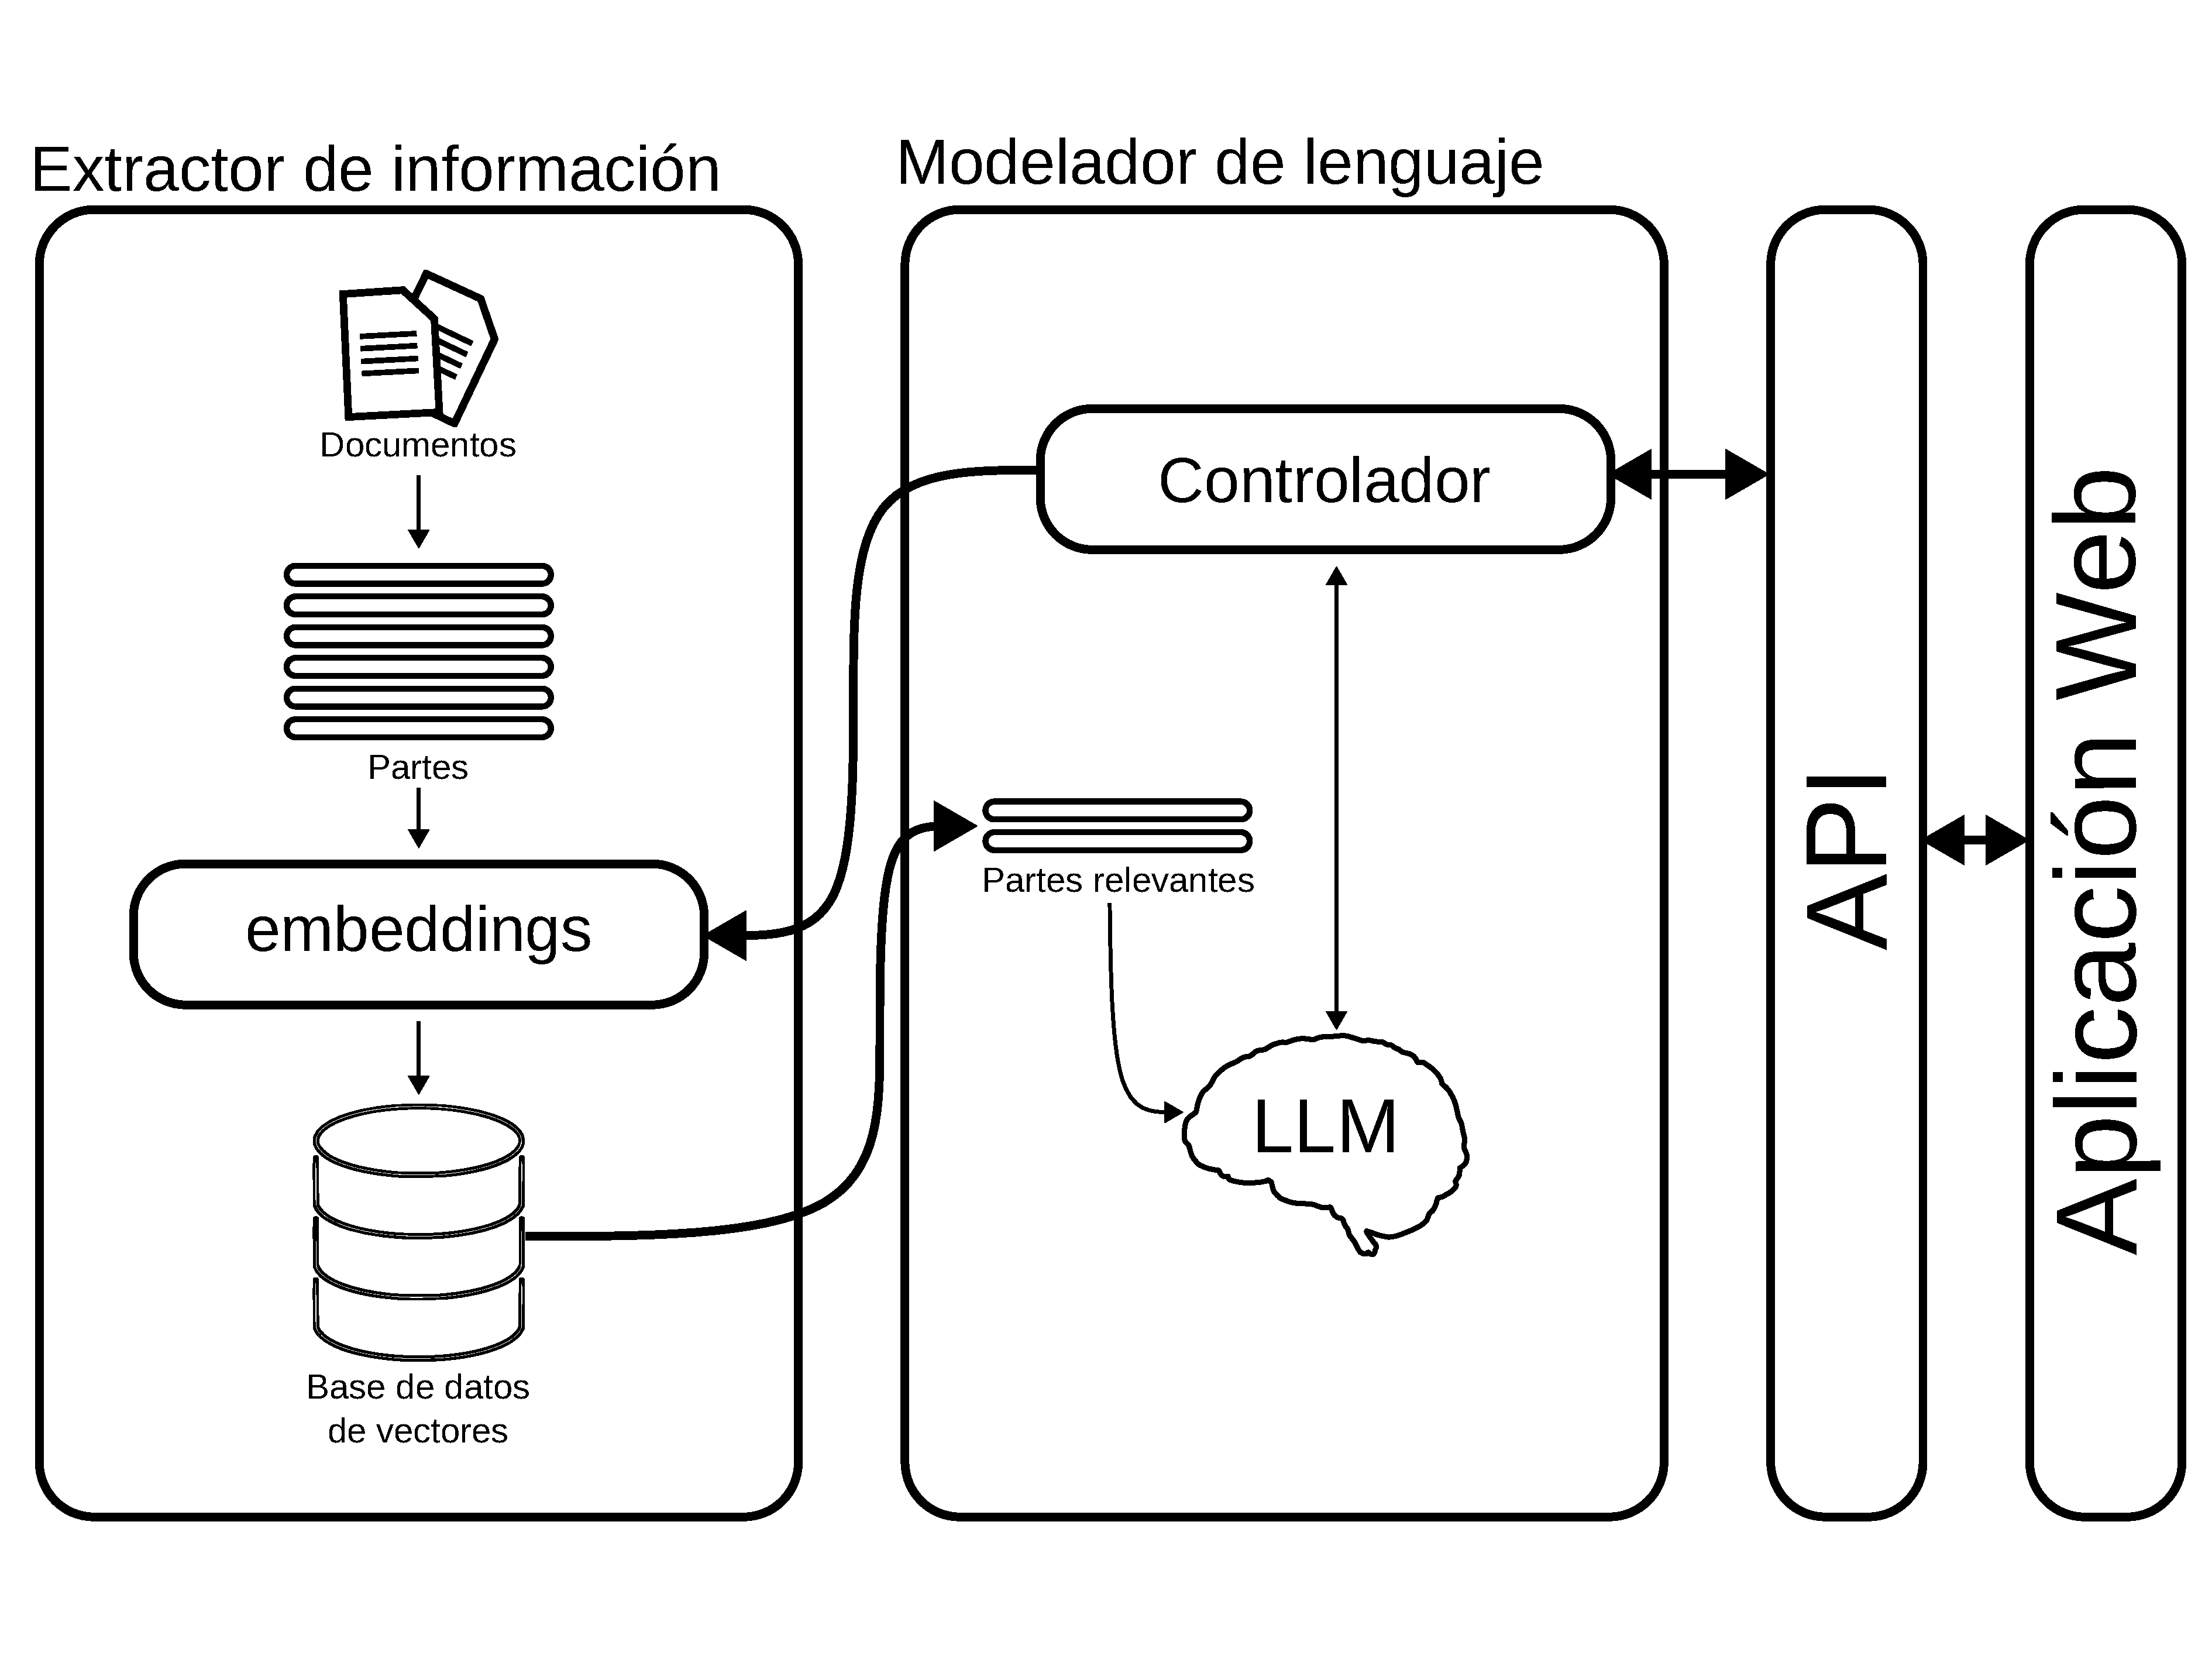
\includegraphics[width = 0.8\textwidth]{\DirFigCtres/esquema_general}
    \caption{Diagrama de componentes que conforman el sistema.}
    \label{fig:esquema_general}
\end{figure}

\section{Fuente de información}

El sistema está diseñado para responder preguntas de la normativa de la
Universidad de Guanajuato, esta normativa se encuentra disponible en la página
oficial de la universidad
\footnote{https://www.ugto.mx/gacetauniversitaria/normatividad/normatividad-vigente}
en forma de 22 documentos PDF individuales. Cada documento tiene un número
diferente de páginas, las cuales suman 511, representan 6.8MB de información y,
convertidas a texto, 168,011 palabras.

Los documentos son descargados manualmente y almacenados en un directorio,
para cada uno se utiliza el nombre del archivo como identificador.

**Incluir tabla con detalle de cada documento de la normativa**

\section{Extractor de información}

El funcionamiento del módulo de extracción de información comienzan con un
archivo en formato PDF y terminan con la creación de una base de datos de
embeddings de los fragmentos del documento. En la figura
\ref{fig:esquema_extractor} se observa la secuencia de procesamiento para un
archivo y la salida de cada una de las etapas.

\begin{figure}[]
    \centering
    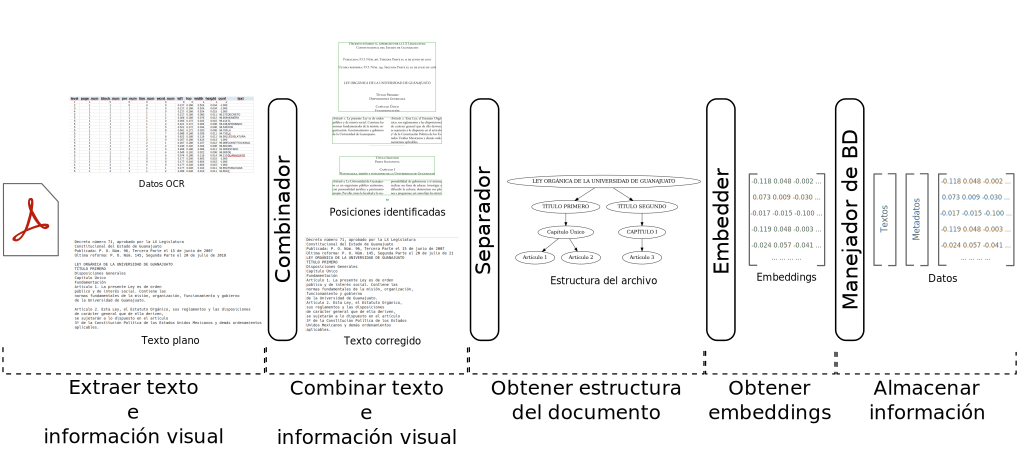
\includegraphics[width = 0.8\textwidth]{\DirFigCtres/esquema_extractor}
    \caption{Diagrama de extracción de información de un archivo PDF.}
    \label{fig:esquema_extractor}
\end{figure}

\subsection{Extraer texto e información visual}

El documento PDF debe convertirse a texto para su procesamiento, pero es
necesario conservar la información del formato y ubicación de los segmentos
para poder extraer la estructura del documento. Por lo anteior, se extraen dos
tipos de datos del archivo: texto plano e información visual relacionada con
el formato.

Para seleccionar las herramientas de extracción de texto plano se hizo un
análisis de aquellas que fueran de código abierto, considerando sus
deficiencias en la extracción de texto (ver Apéndice A). Se seleccionaron
PyPDF, porque es la herramienta más usada para esta tarea con Python, y
PdfPlumber, porque su extracción de texto es la más limpia y provee mecanismos
para extraer la información visual.

Primero se extrae el texto plano con PyPDF o PdfPlumber. En el caso de PyPDF
no se obtiene información visual que ayude a identificar los títulos, secciones
y encabezados, además en ocasiones modifica el orden del texto. Cuando se
emplea PdfPlumber, el texto va acompañado de la información visual del docuemto,
que consiste en la ubicación de cada palabra dentro del docuemnto.

Para obtener la información visual, cuando no se tiene, se utiliza la herramienta
Tesseract, la cual es un software de reconocimiento óptico de caracteres que
nos permite obtener la ubicación y texto de cada palabra dentro del documento.
Para emplear Tesseract, primero se convierte el documento a imágenes con
PDF2Image, las imágenes resultantes tienen una densidad de pixeles de 1000 DPIs.
Posteriormente, se usa la librería PyTesseract para obtiener información del
documento, específicamente, para cada palabra de la página obtiene: posición,
ancho, alto y texto predicho.

La librería PyTesseract ejecuta la herramienta Tesseract, desarrollada por
Google para hacer OCR. Esta herramienta puede reconstruir el texto del documento,
así como detectar las líneas, párrafos y secciones, sin embargo, con frecuencia
comete errores en la detección del texto y el ordenamiento. Para corregir
estos errores se opta por combinar el texto plano obtenido con PyPDF, con
la información de posición y tamaño devuelto por PyTesseract, de esta forma
obtenemos el texto correcto asociado a su ubicación y tamaño. Este proceso
se describe en el diagrama de la figura \ref{fig:texto_y_ocr}.

\begin{figure}[]
    \centering
    \includegraphics[width = 0.8\textwidth]{\DirFigCtres/esquema_texto_y_ocr}
    \caption{Detalle extracción de texto y características de OCR.}
    \label{fig:texto_y_ocr}
\end{figure}

Para el caso de PdfPlumber, la librería devuelve las mismas características que
PyTesseract, sin embargo, comete también errores en la agrupación y el
ordenamiento del texto, por ello se requiere realizar los pasos de "Crear
grupos para reconstruir el texto" y "Reconstruir texto" del diagrama de la figura
\ref{fig:texto_y_ocr}.

La tarea de agrupar el texto en secciones para reconstruirlo en el orden correcto
no es trivial, y es altamente dependiente del tipo de documento del
que se trata, es decir, el proceso descrito en el diagrama de las figuras
\ref{fig:reconstruccion_texto_1} y \ref{fig:reconstruccion_texto_2} funciona para
documentos con estructura similar, donde predomina el texto en una o dos
columnas con títulos centrados.

\begin{figure}[]
    \centering
    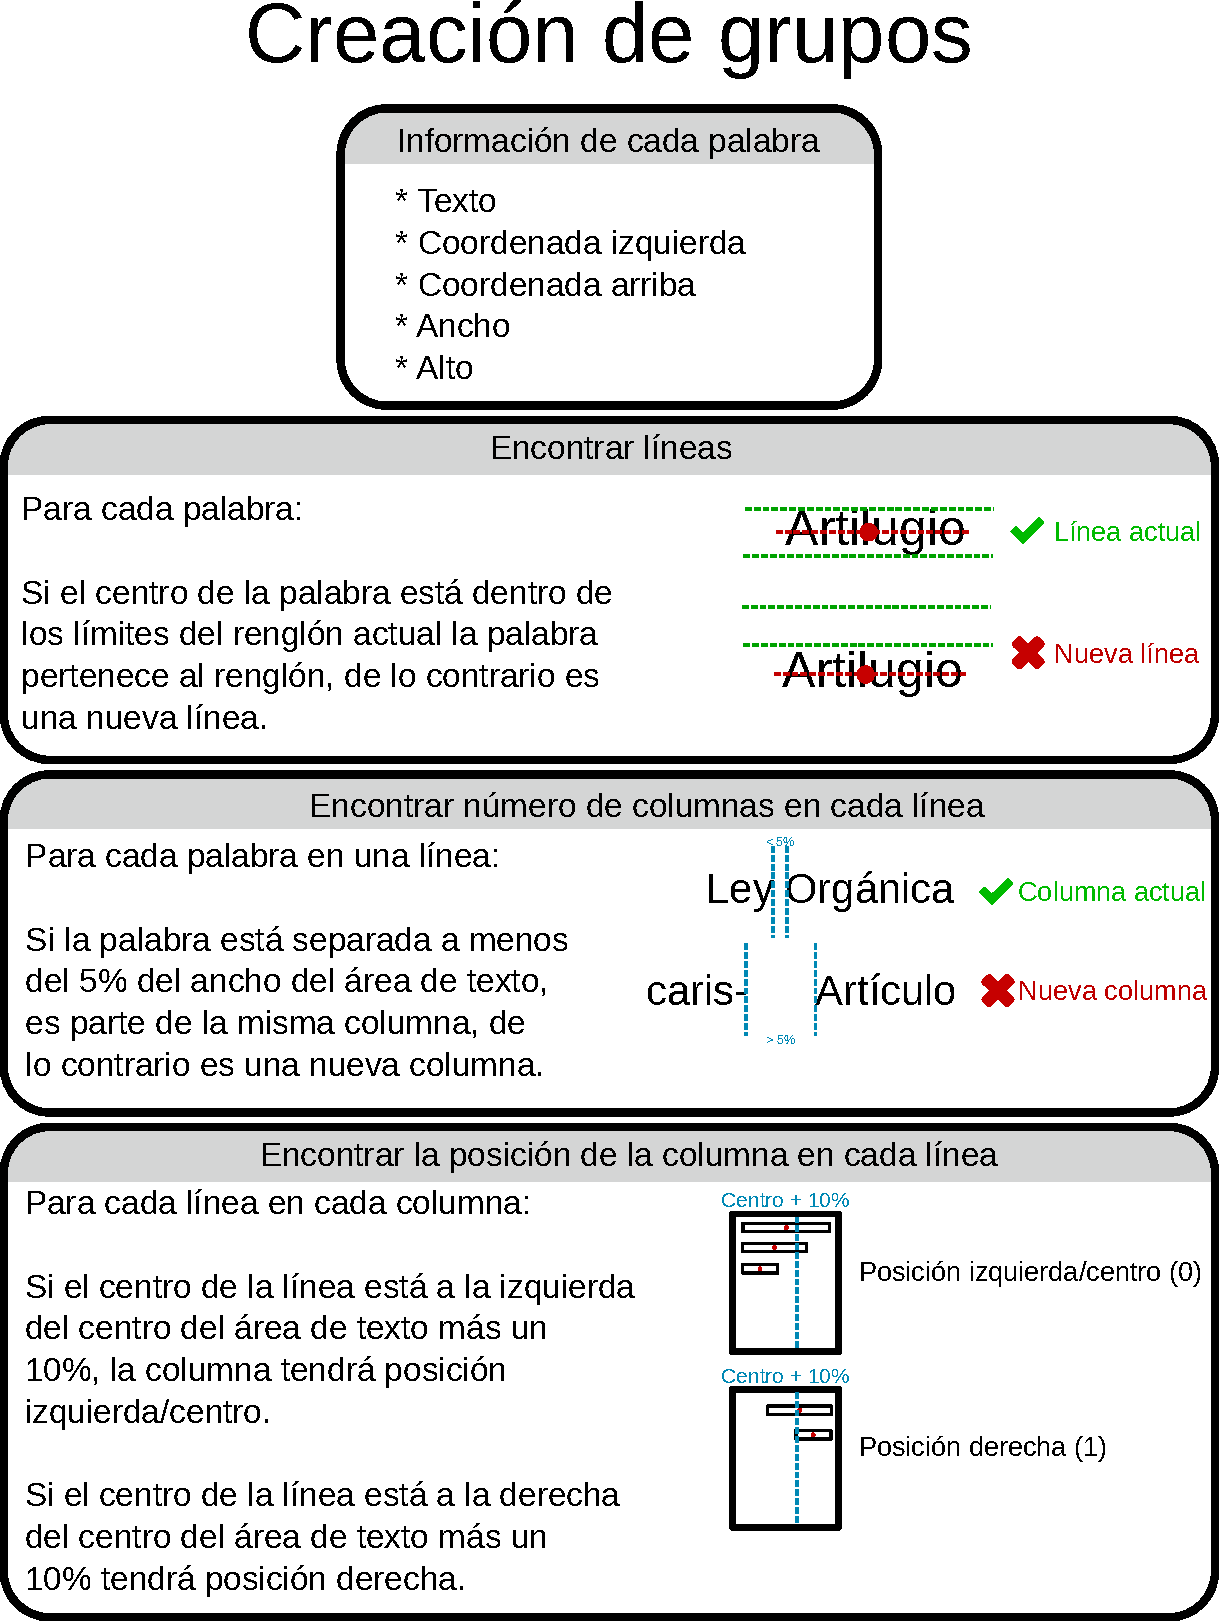
\includegraphics[width = 0.8\textwidth]{\DirFigCtres/reconstruccion_texto_ocr_1}
    \caption{Detalle de reconstrucción de texto del documento (Pt. 1).}
    \label{fig:reconstruccion_texto_1}
\end{figure}

\begin{figure}[]
    \centering
    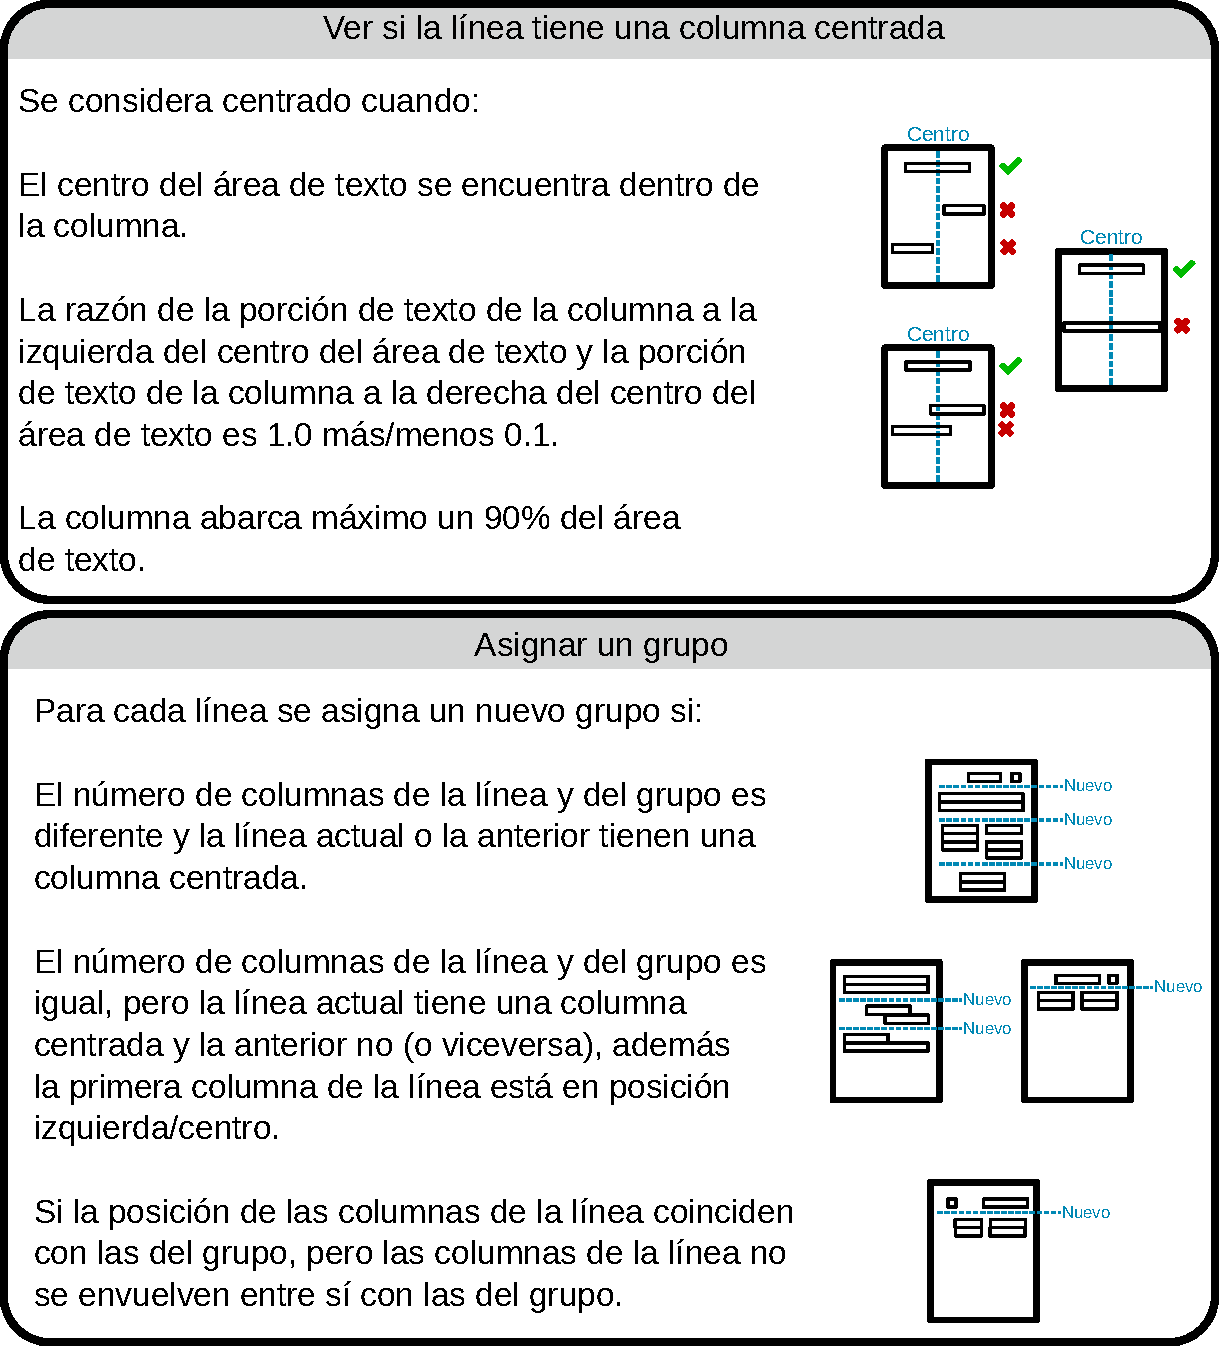
\includegraphics[width = 0.8\textwidth]{\DirFigCtres/reconstruccion_texto_ocr_2}
    \caption{Detalle de reconstrucción de texto del documento (Pt 2).}
    \label{fig:reconstruccion_texto_2}
\end{figure}

Una vez realizada la agrupación de los elementos de la página, es posible reconstruir
el texto respetando el orden normal de lectura. Este texto usualmente contiene
errores de detección que serán corregidos al combinar el texto reconstruido
con OCR con el texto plano extraido con PyPDF.

\subsection{Combinar texto e información visual}

Cuando se usa PdfPlumber, este proceso no es necesario, pues la librearía ya
devuelve el texto correcto asociado a su informació visual de posición y tamaño,
sin embargo, cuando se usa PyPDF y PyTesseract, es necesario combinar estas dos
fuentes de información para obtener el texto e información visual correctas,
el objetivo es tener la posición de cada palabra asociada con su texto correcto,
de esta forma se podrá distinguir entre diferentes elementos, como títulos,
párrafos, entre otros.

El proceso de combinación requiere las cadenas de texto extraídas por los dos métodos:
la cadena proporcionada por PyPDF y la cadena reconstruida con la información
visual, como se muestra en la figura \ref{fig:reconstruccion_texto_2}. Ambas cadenas se
separan por palabra y se pasan a la librería Difflib, la cual aplica el algoritmo
Ratcliff-Obershelp, también conocido como Coincidencia de patrones Gestalt, para
comparar dos cadenas y encontrar sus diferencias.

Si se analizan los patrones de salida de la librería Difflib, es posible
corregir las palabas detectadas con OCR utilizando las palabras extraidas directamente
del texto, los detalles de esta implementación se explican en las figuras
\ref{fig:esquema_combinacion_txt_ocr_1} y \ref{fig:esquema_combinacion_txt_ocr_2}.
En escencia, se considera la palabra obtenida con PyPDF como la correcta,
se compara contra la palabra obtenida con OCR y si es diferente se sobreescribe.

\begin{figure}[]
    \centering
    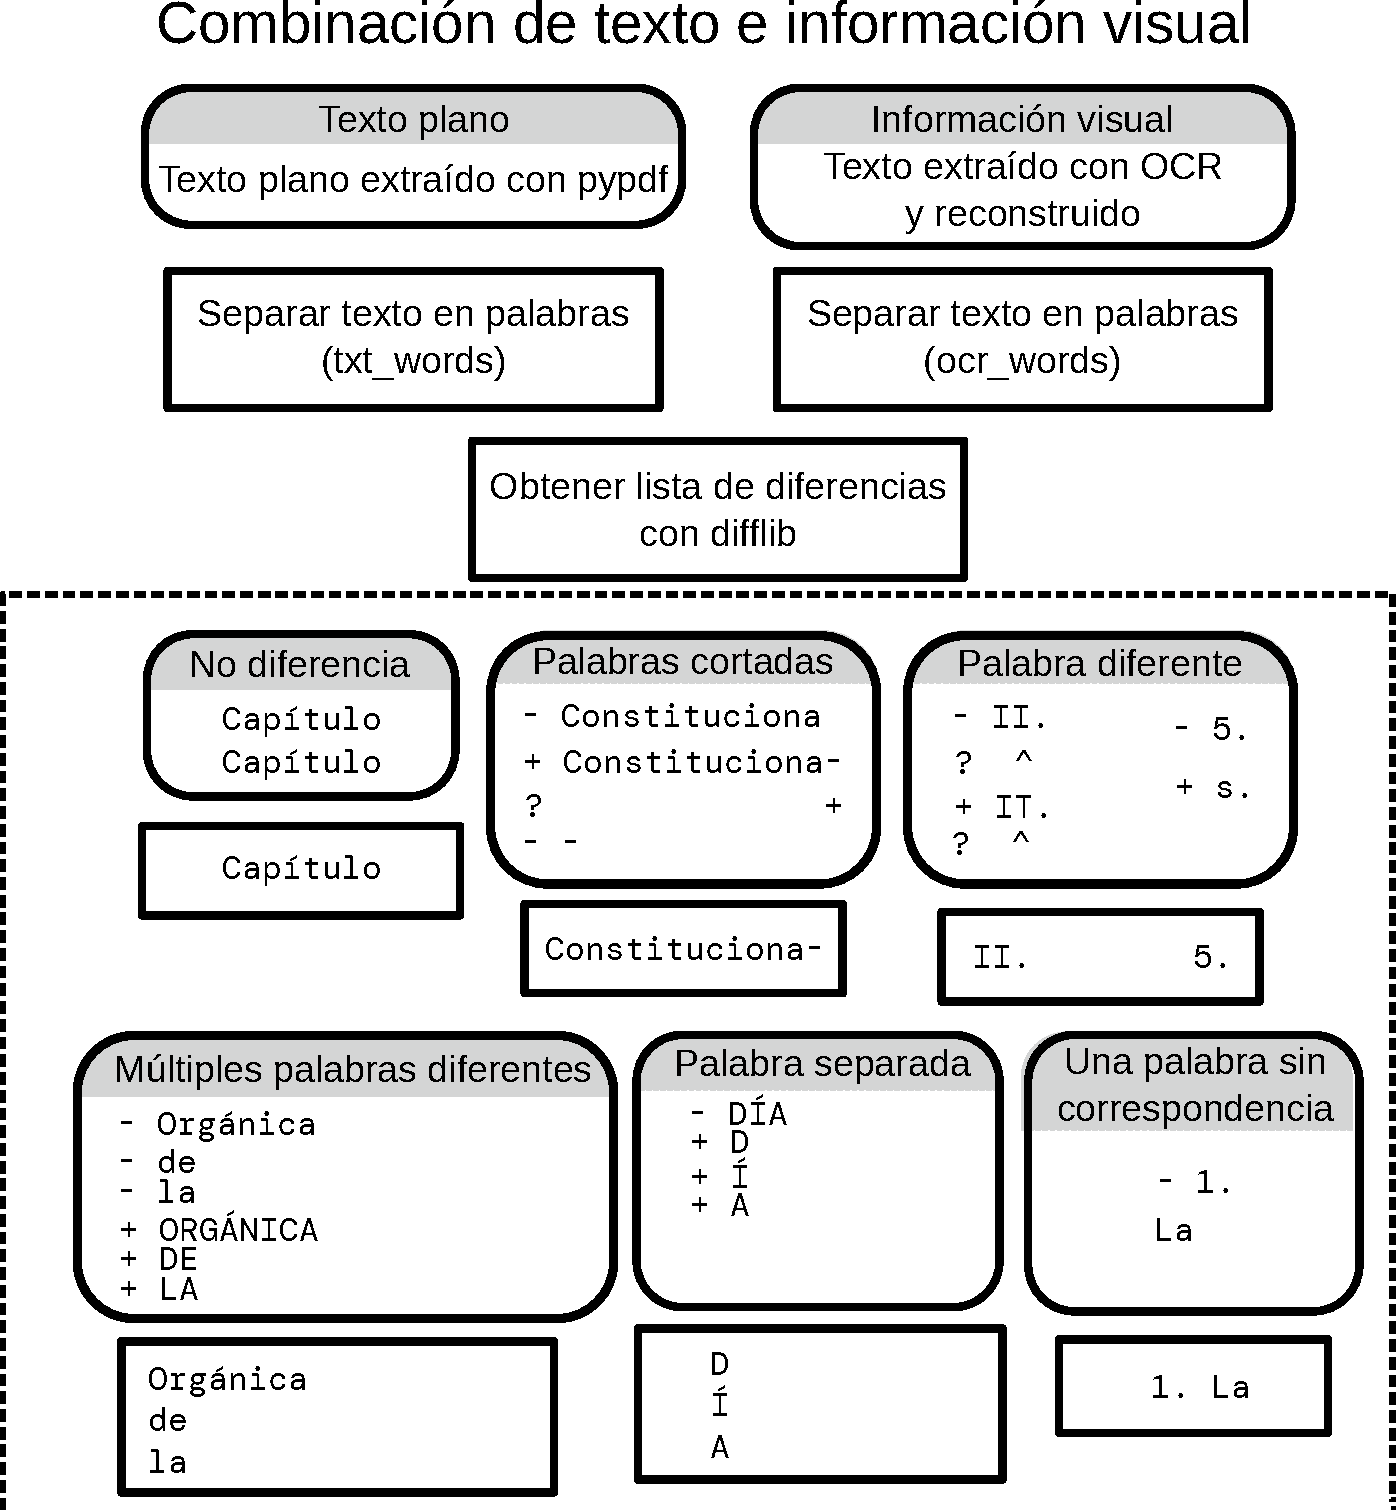
\includegraphics[width = 0.8\textwidth]{\DirFigCtres/combinacion_texto_ocr_1}
    \caption{Detalle de combinación de teto plano con información de OCR (Pt 1).}
    \label{fig:esquema_combinacion_txt_ocr_1}
\end{figure}

\begin{figure}[]
    \centering
    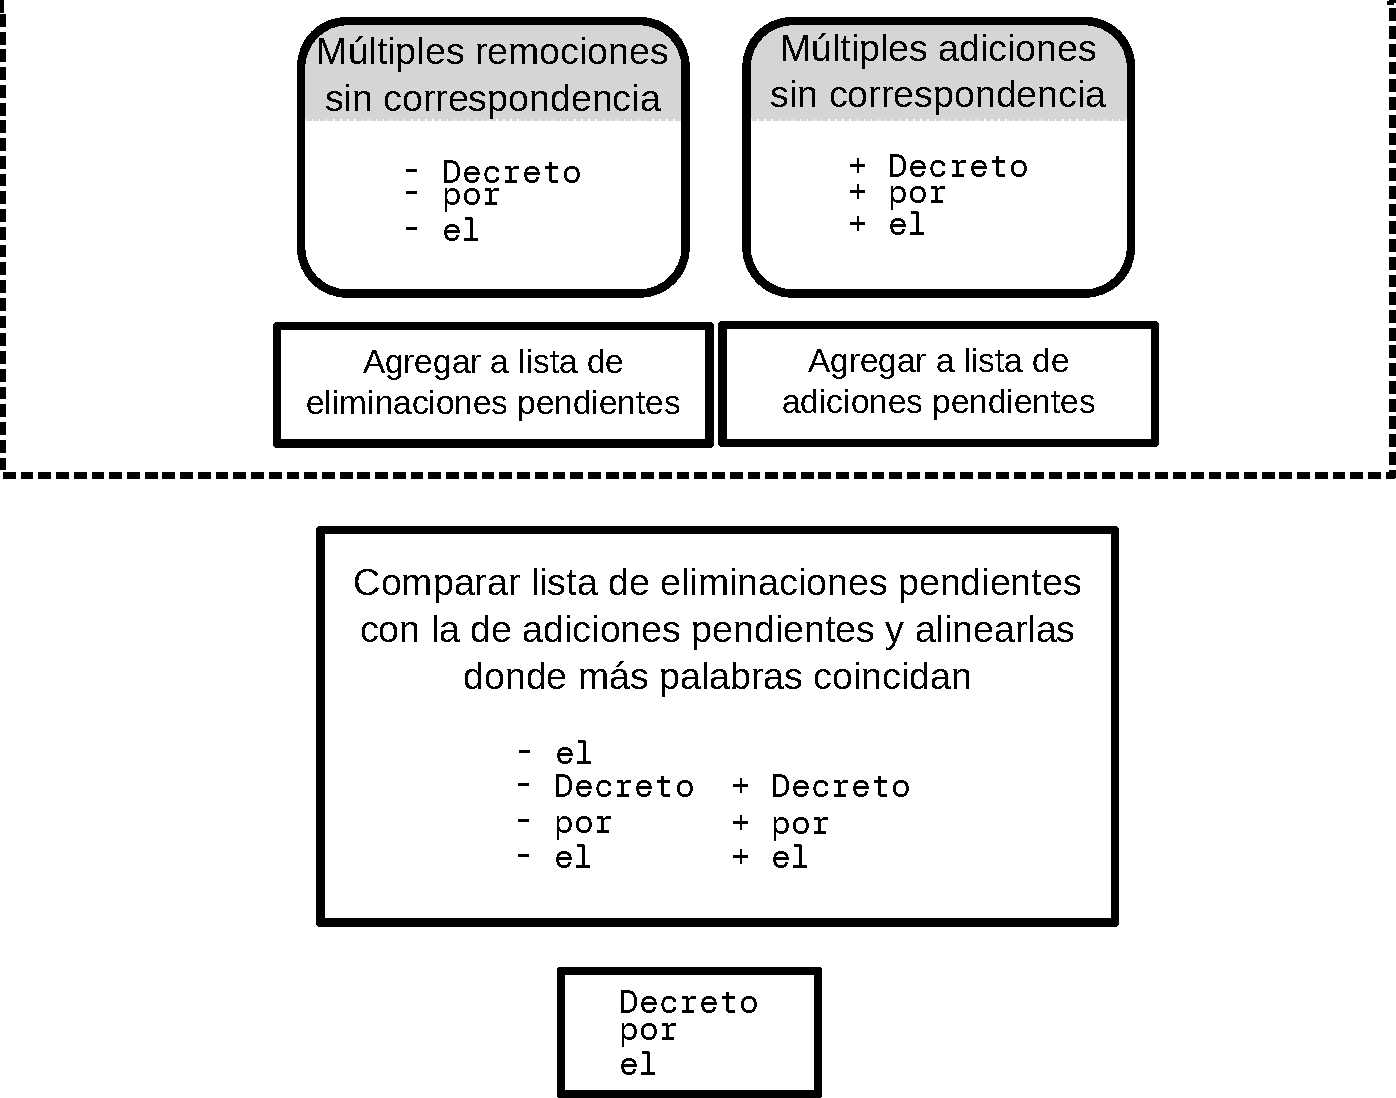
\includegraphics[width = 0.8\textwidth]{\DirFigCtres/combinacion_texto_ocr_2}
    \caption{Detalle de combinación de teto plano con información de OCR (Pt 2).}
    \label{fig:esquema_combinacion_txt_ocr_2}
\end{figure}

Al terminar el proceso se tiene un arreglo de datos donde se conoce la posición
y dimensiones de cada palabra, así como su texto correcto, además se cuenta con
datos adicionales de linea, columna, alineación o grupo que serán empleadas
para dividir las secciones del documento más adelante.

Las ventajas de usar PdfPlumber sobre PyPDF+PyTesseract son que es más rápido y
la identificación del texto es certera, pues proviene directamente del archivo,
sin embargo, no funciona si el PDF es un escaneo o si contiene texto en forma
de imagen.

Por su parte, al generar el método que emplea PyPDF+PyTesseract, se desarrollaron
elementos que fueron reciclados, como la resconstrucción de texto, además de
que puede funcionar en documentos escaneados (confiando completamente en la
predicción de PyTesseract) y documentos con imágenes, además de que es mejor
eliminando texto no visible en el PDF.

\subsection{Obtener estructura del documento}

El objetivo de este paso es generar una estructua de datos en la que cada parte
del documento esté referenciada a su sección y subsecciones correspondientes,
por ejemplo, para la Ley Orgánica deseamos conocer en qué título, capítulo y
artículo se encuentra un texto específico.

Para realizar dicha estructura se optó por generar un árbol, donde cada nodo
corresponde a una sección del documento, además, las hojas y los nodos intermedios
almacenan el texto de cada artículo o sección según sea el caso. En la figura
\ref{fig:fragmento_arbol} se muestra un fragmento del árbol correspondiente a
las primeras secciones de la Ley Orgánica.

\begin{figure}[]
    \centering
    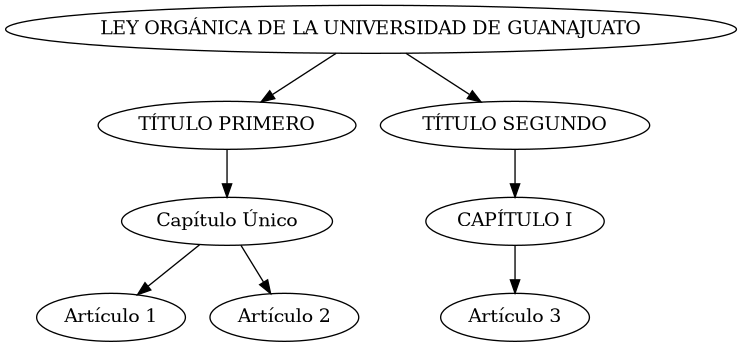
\includegraphics[width = 0.8\textwidth]{\DirFigCtres/fragmento_arbol}
    \caption{Fragmento de árbol de documento 'Ley Orgánica de la Universidad de Guanajuato'.}
    \label{fig:fragmento_arbol}
\end{figure}

Para generar el árbol es necesario analizar el documento en varios pasos. Primero,
se detectan las líneas o fragmentos que corresponden a títulos, estas típicamente
se encuentran centrados en la página o en la columna, a los primeros se les
asigna el tipo 1 y a los segundos el tipo 2, el texto restante tendría tipo 0.
Para que el fragmento sea considerado como título deberá haber un espacio
vertical antes o después dependiendo del tipo.

Para encontrar las secciones o subsecciones se consideran los títulos
centrados en la página (tipo 1), a los cuales se les asigna un nivel. Para asignar
el nivel a un título es necesario conocer de antemano la estructura del
documento, específicamente, se debe crear una expresión regular para
identificar cada nivel. Por ejemplo, para la Ley Orgnánica de la Universidad
de Guanajuato la estructura que se tiene es la siguiente:

\begin{enumerate}
    \item Encabezado general: Son títulos abiertos que no tienen palabras o
          estructura específica y se consideran dentro del primer nivel.
          \begin{itemize}
              \item Sin expresión regular
          \end{itemize}
    \item Título: El documento se divide en títulos. Cada título comienza con
          la palabra \textit{Título}.
          \begin{itemize}
              \item \string^(título\textbar[xiv]+\textbackslash.) .*
          \end{itemize}
    \item Capítulo: Los títulos se dividen an capítulos y cada capítulo comienza
          con la palabra \textit{Capítulo}
          \begin{itemize}
              \item \string^capítulo .*
          \end{itemize}
\end{enumerate}

Además, se debe tener en cuenta que hay divisiones del documento
que no se encuentran centrados, sino que están contenidos en el grueso del
texto, como lo son los Artículos. Para identificar estas separaciones en el
contenido, también se crean expresiones regulares que se verifican contra el
inicio de cada línea mientras se va construyendo el árbol.

\begin{enumerate}
    \item Artículo: Los capítulos tienen uno o más artículos.
          \begin{itemize}
              \item  \string^artículo ([0-9]+\textbar[a-zé]+(ro\textbar do\textbar ro\textbar to\textbar mo\textbar vo\textbar no\textbar único)\\
                    (bis\textbar ter\textbar quáter\textbar quinquies)?\textbackslash.
          \end{itemize}
\end{enumerate}

Una vez identificados los títulos y teniendo la forma para encontrar las
divisiones dentro del contenido, se recorre el documento. Recorrer
el documento es el equivalente a recorrer el árbol por profundidad, por lo
que se va creando el árbol de la misma forma, es decir, cuando se encuentra
un título se crea un nuevo nodo en el nivel correspondiente, siempre teniendo
la referencia de cual será su padre, cuando se llega al nivel más bajo se
guarda el contenido de texto en el nodo correspondiente.
El proceso completo se presenta en la figura
\ref{fig:crear_arbol}.

\begin{figure}[]
    \centering
    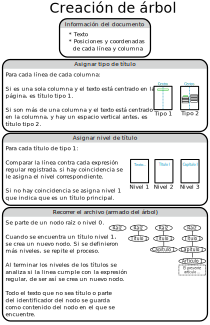
\includegraphics[width = 0.8\textwidth]{\DirFigCtres/crear_arbol}
    \caption{Proceso de creación del árbol de secciones de un documento.}
    \label{fig:crear_arbol}
\end{figure}

\subsection{Obtener \textit{embeddings}}

Para el cálculo de \textit{embeddings} se emplean LLMs especializados,
estos modelos son entrenados en datasets de similitud semántica o QA en
diferentes idiomas. El sistema propuesto permite el uso y evaluación de
varios modelos, los cuales serán: MiniLM (33M de parámetros)
\cite{wang_minilm_2020}, MPNET \cite{hagen_mpnet_2020} (110M de parámetros)
y Qwen 3 \cite{zhang_qwen3_2025} (600M, 4B y 8B de parámetros). Estos modelos
se encuentran disponibles en HuggingFace para su descarga y se pueden
emplear a través de la librería \textit{SentenceTransformers}, la cual está especializada
en obtener embeddings de oraciones.

Los modelos MiniLM y MPNET fueron seleccionados por su tamaño reducido,
ya que incluso pueden correr en CPU de forma eficiente, mientras que los
modelos Qwen fueron seleccionados porque ocupan los primeros puestos en el
MTEB Ladderboard de HuggingFace \footnote{https://huggingface.co/spaces/mteb/leaderboard},
que clasifica modelos de extracción de \textit{embeddings} en diferentes idiomas
y con múltiples métricas.

En el caso de los modelos Qwen 3, existen versiones cuantizadas de éstos,
las cuales emplean el mismo número de parámetros que su versión original,
pero disminuyendo la precisión de los números flotantes de sus parámetros.
Para el caso de Qwen 3, existen versiones de 16-bits, 8-bits, 6-bits, 5-bits y
4-bits.

**Incluir tabla resumen de modelo, parámetros y tamaño de embeddings.**

El proceso para convertir la información del documento a embeddings consiste
en recorrer el árbol en profundidad, y en cada nodo hacer lo siguiente:

\begin{enumerate}
    \item Tomar el contenido textual del nodo y separarlo por párrafos.
          Cada párrafo será un registro independiente.
    \item Utilizar SentenceTransformers para calcular los embeddings de cada
          párrafo y guardarlo como un vector de números.
    \item Obtener la ruta del nodo dentro del árbol. Ej: Ley Orgánica $\rightarrow$
          Título Primero $\rightarrow$ Capítulo segundo $\rightarrow$ Artículo 30.
    \item Guardar la ruta y el nombre del nodo como metadatos (información
          adicional que se podría usar para filtrar la información).
\end{enumerate}

Al final por cada párrafo del documento se tendrá la siguiente información:

\begin{itemize}
    \item Metadatos:
          \begin{itemize}
              \item Ruta en el árbol
              \item Nombre del nodo
          \end{itemize}
    \item Embedding como vector de N valores numéricos.
\end{itemize}

\subsection{Almacenar información}

Los embeddings pueden almacenarse de varias formas en el disco, sin embargo,
las dos formas más convenientes son: en formato CSV o en una base de datos
que soporte vectores.

El formato CSV tiene la ventaja de ser portable y facil de leer, lo único que
hay que hacer es convertir los metadatos a formato JSON, así podrán ser
almacenados como texto, mientras que el vector de embeddings se puede
expandir y crear una columna para cada valor. En la figura \ref{fig:ejemplo_csv}
se muestra un ejemplo de la información almacenada como archivo CSV.

\begin{figure}[]
    \centering
    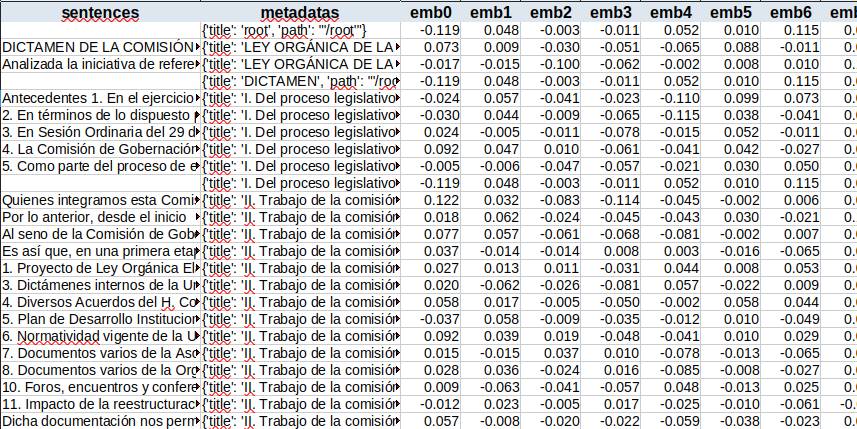
\includegraphics[width = 0.8\textwidth]{\DirFigCtres/ejemplo_csv}
    \caption{Ejemplo de cómo se almacenan metadatos y embeddings en formato csv.}
    \label{fig:ejemplo_csv}
\end{figure}

Sin embargo, este método no es apto para entornos productivos, ya que no tiene
mecanismos nativos para búsqueda en los vectores de datos.

Otra forma de almacenar los embeddings es empleando una base de datos que
soporte vectores. Existen muchas alternativas y cada una ofrece beneficios
particulares, en general todas permiten almacenar los datos de forma
óptima ya que se pueden organizar en tablas, agregar informació adicional y
tienen implementadas funciones de búsqueda por similitud de vectores.
Algunos ejemplos de estas bases de datos vectoriales son: Chroma, Marco,
PostgreSQL, entre otras.

ChromaDB es una base de datos de vectores diseñada para funcionar en
entornos productivos, e incluye mecanismos para calcular los embeddings
empleando \textit{SentenceTransformers} u otro método personalizado, además,
permite el uso de diferentes parámetros de búsqueda por similitud semántica
como son la distancia coseno y el producto interno, los cuales también se
encuentran optimizados. En la figura \ref{fig:ejemplo_chromadb} se muestra
un ejemplo de datos almacenados en ChromaDB.

\begin{figure}[]
    \centering
    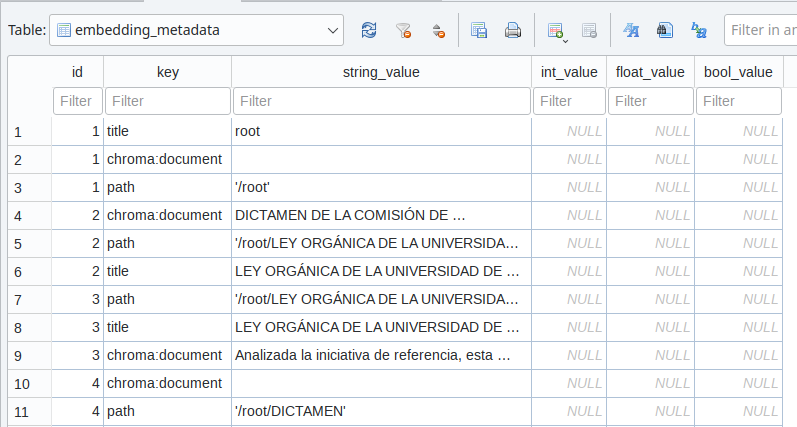
\includegraphics[width = 0.8\textwidth]{\DirFigCtres/ejemplo_chromadb_1}
    \caption{Ejemplo de cómo se almacenan metadatos en Chroma DB. Los vectores
        se almacenan en un lugar no visible para el usuario.}
    \label{fig:ejemplo_chromadb}
\end{figure}

\section{Modelador de lenguaje}

El modelador de lenguaje tiene dos funciones fundamentales: manejar la
interacción con la base de datos de vectores y manejar la interacción con el
LLM principal, en términos de RAG, se encarga de la recuperación y la
generación.

El proceso general que ejecuta el modelador de lenguaje se presenta en el
diagrama de la figura \ref{fig:esquema_modelador} y se explica a continuación.

\begin{figure}[]
    \centering
    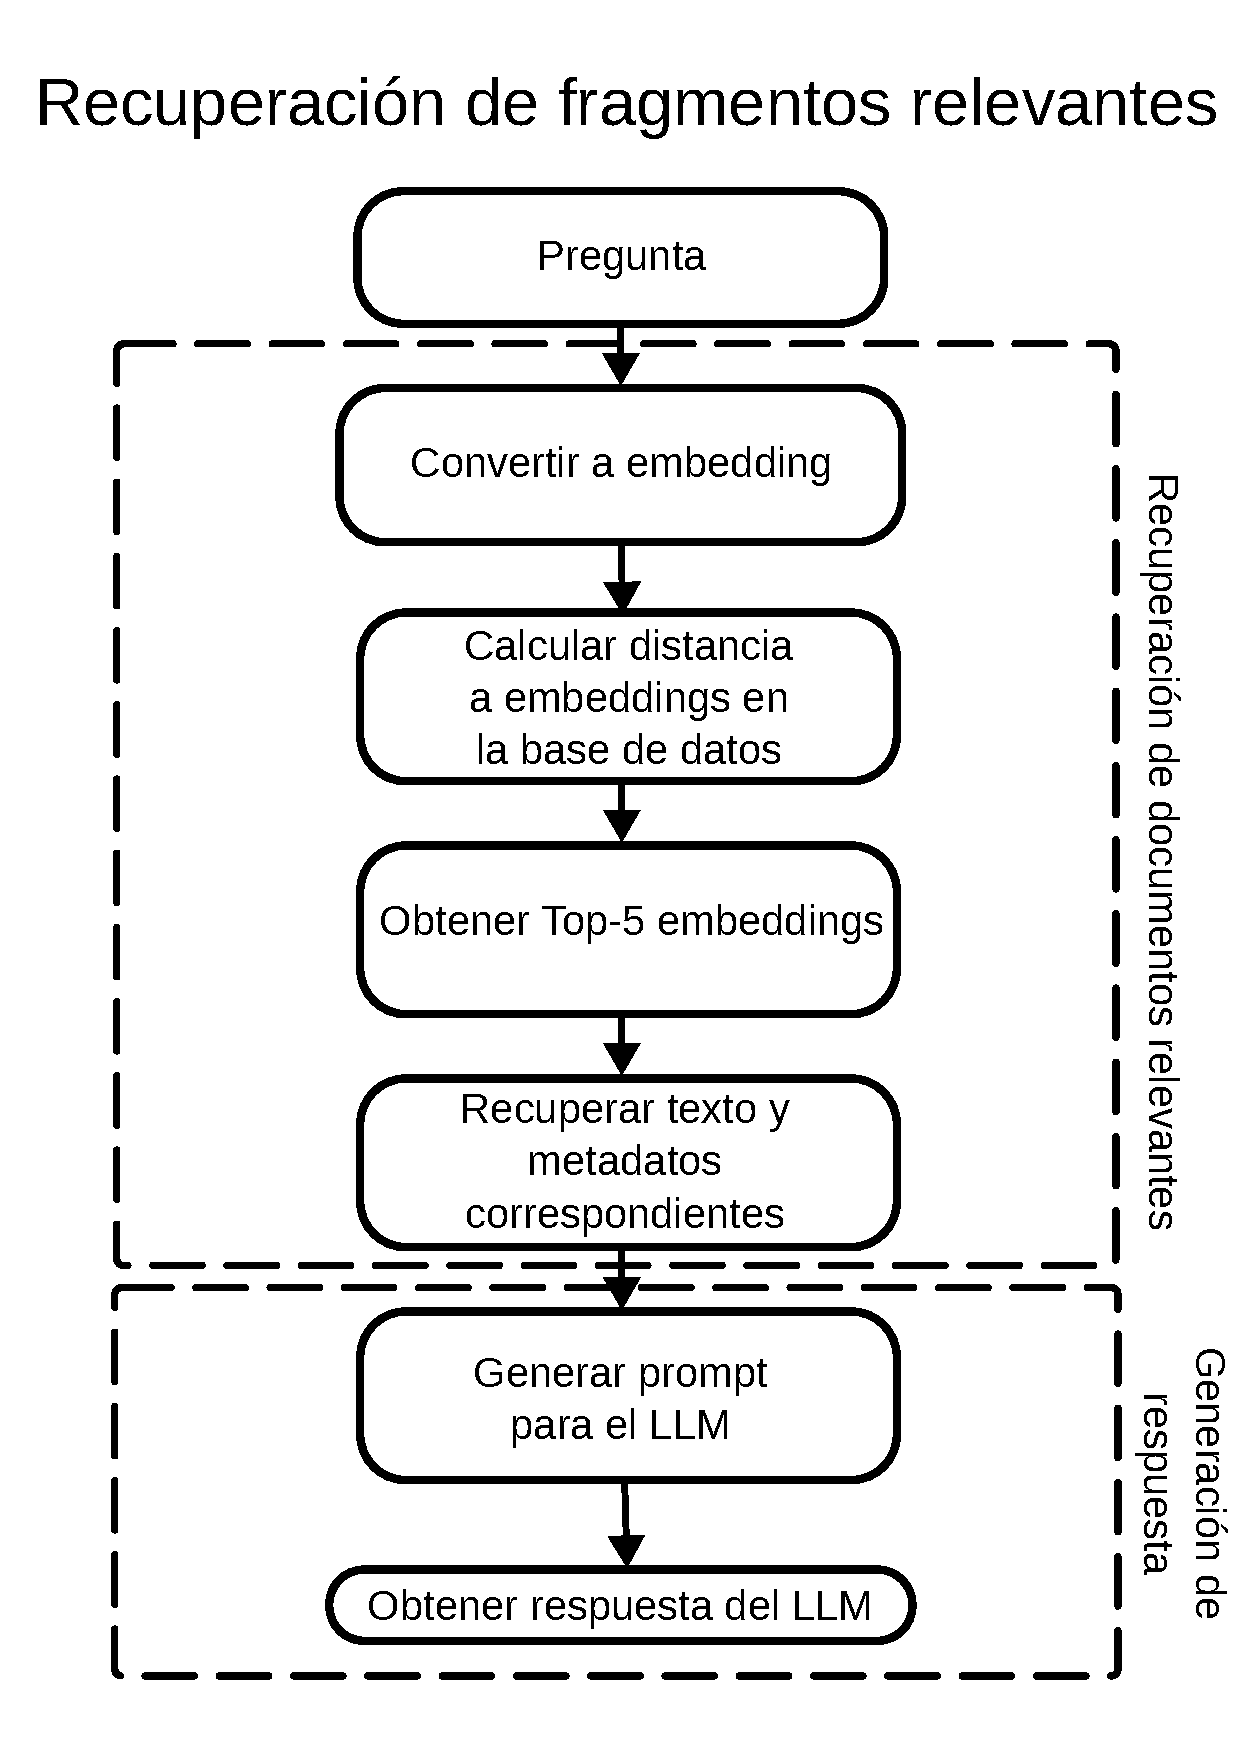
\includegraphics[width = 0.8\textwidth]{\DirFigCtres/esquema_recuperacion}
    \caption{Pasos seguidos por el modelador de lenguaje para procesar una pregunta.}
    \label{fig:esquema_modelador}
\end{figure}

\subsection{Recuperación de documentos relevantes}

Dada una pregunta o \textit{query}, el modelador la convierte a \textit{embedding}
empleando el mismo modelo usado para la base de datos. Este \textit{embedding}
se le proporciona a ChromaDB para hacer la búsqueda semántica, el parámetro
de búsqueda puede ser por producto interno o por similitud coseno, dependiendo
del modelo de \textit{embeddings}. Para hacer una búsqueda eficiente,
ChromaDB emplea un índice llamado HNSW (Hierarchical Navigable Small World),
esto le permite buscar de forma eficiente la similitud con todos los registros.

Con ChromaDB se obtiene el top \textit{k} de \textit{embeddings} similares,
por defecto \textit{k} se establece en 5. De estos \textit{k} \textit{embeddings}
se obtiene su texto original, su posición dentro del árbol del documento, el
documento al que pertenece y los demás metadatos.

\subsection{Generación de respuesta}

Para la generación de la respuesta, se emplean modelos multidominio de código
abierto, la intención es comparar modelos de diferentes tamaños para
encontrar el óptimo. Se evaluan los modelos Qwen 3 \cite{zhang_qwen3_2025}
(600M, 4B y 8B de parámetros) en sus versiones completas y cuantizadas,
Llama 3.1 (1B, 3B y 8B de parámetros) en sus versiones completas y cuantizadas
y Gemma 3 (1B, 4B, 12B y 27B de parámetros) en sus versiones completas y
cuantizadas.

**Agregar tabla comparativa de modelos**

A todos los modelos se les configura una instrucción de sistema indicando
que su propósito es proporcionar ayuda sobre la normativa y se le indican
algunos lineamientos de comportamiento.

**Agregar prompt del sistema con instrucciones**

Una vez se tiene una pregunta y sus los fragmentos relevantes, se extrae
tanto el texto como sus metadatos, los cuales incluyen: el documento, artículo
o sección, y, en algunos casos, el subtítulo o nombre de sección.
Con el fin de transmitir esta información al LLM, se crea una plantilla de
\textit{prompt} que contiene la pregunta, los documentos relevantes y la
instrucción de responder la pregunta con el contexto proporcionado.

**Agregar plantilla del prompt.**

Una vez generado el \textit{prompt} se le manda al LLM, junto con el historial
anterior del chat en caso de existir, y se espera por la respuesta.

\section{API de comunicación}

**Reemplazar esta sección con la documentación formal de la API**

La tarea de la API es conectar la aplicación web con el modelador de lenguaje.
La API funciona con peticiones http de tipo POST y conste en un solo endpoint
el cual recibe el nombre del modelo y la lista de mensajes entre el
usuario y el modelo, cada mensaje se identifica con un rol para distinguir
los mensajes del usuario de las respuestas del modelo. Las peticiones se
manejan en formato JSON como se muestra en la figura \ref{fig:parametros_api}.

\begin{figure}[]
    \centering
    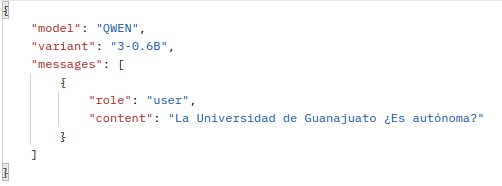
\includegraphics[width = 0.8\textwidth]{\DirFigCtres/parametros_api}
    \caption{Ejemplo de petición a API.}
    \label{fig:parametros_api}
\end{figure}

La respuesta de la API también es en formato JSON y contiene el texto de la
respuesta, así como los documentos que fueron tomados como contexto para
emitirla, como se muestra en la figura \ref{fig:respuesta_api}. En estos
documentos, se incluyen los metadatos para poder desplegarlos en la aplicación
web.

\begin{figure}[]
    \centering
    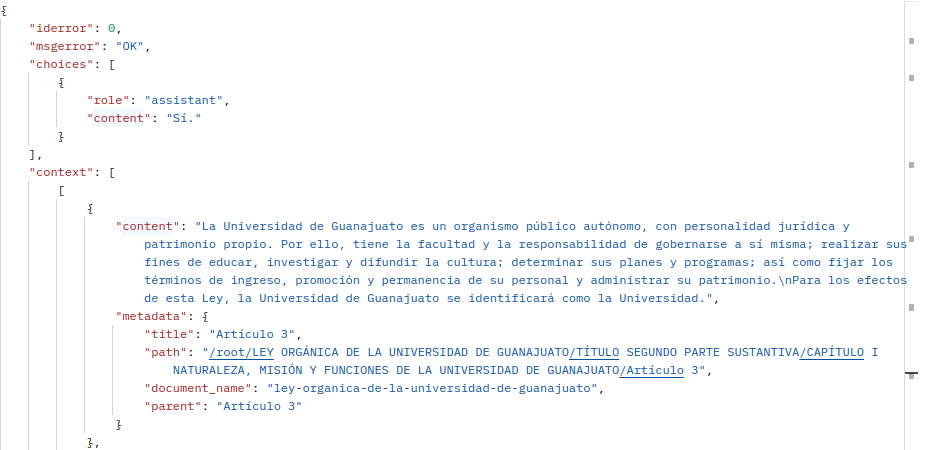
\includegraphics[width = 0.8\textwidth]{\DirFigCtres/respuesta_api}
    \caption{Ejemplo de respuesta de API.}
    \label{fig:respuesta_api}
\end{figure}

Por último, para garantizar la seguridad en el acceso de la API, se implementa
un sistema de autenticación por API-Key, la cual es un token que debe
enviarse en el encabezado 'api-key' de la petición.

\section{Aplicación web}

La aplicación web es la única fuente de interacción de los usuarios con el
sistema, es por ello que debe contener todas las funcionalidades necesarias
que en este caso son: Ingresar una pregunta, recibir una respuesta y
consultar los documentos que dan fundamento a dicha respuesta.

Es bajo esta premisa que se desarrolla una aplicación web con una interfaz
que contiene una caja de texto para hacer la pregunta y despliega la
lista de mensajes y respuestas como un chat convencional. Adicionalmente
se destina un espacio para colocar los documentos relacionados con la
pregunta, como se muestra en la figura \ref{fig:pregunta_web}.

\begin{figure}[]
    \centering
    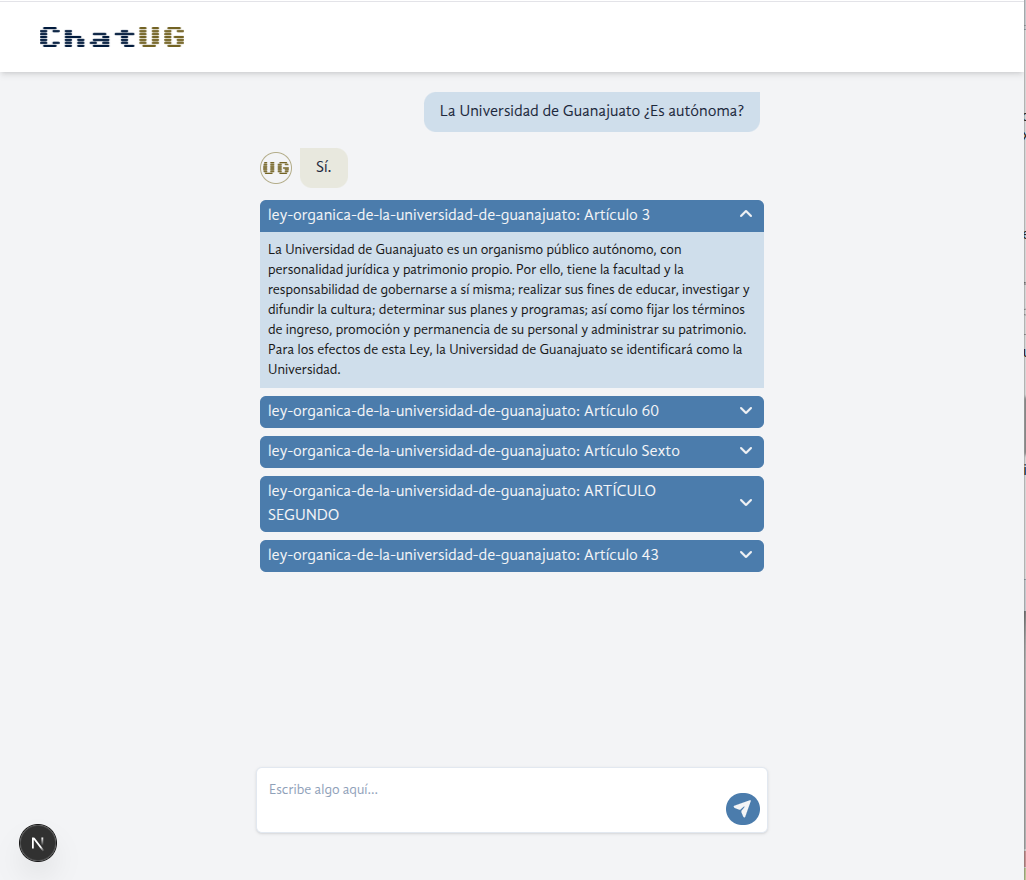
\includegraphics[width = 0.8\textwidth]{\DirFigCtres/pregunta_web}
    \caption{Ejemplo de pregunta a través de aplicación web. **Reemplazar
        esta imagen con el wireframe o prototipo de la aplicación**}
    \label{fig:pregunta_web}
\end{figure}

%\input{./Chapters/Capitulo4}
%\input{./Chapters/Conclusiones}
%\addcontentsline{toc}{chapter}{Conclusiones.}

%%%%%%%%%%%%%%%%%%%%%%%     Apéndices     %%%%%%%%%%%%%%%%%%%%%%%
%\appendix
%\input{./Chapters/planos}
%\input{./Chapters/SRF02}

%%%%%%%%%%%%%%%%%%%%%%%     Bibliografía     %%%%%%%%%%%%%%%%%%%%%%%

\bibliography{./Biblio/Bibliography}    		% Se agrega la bibliografía
\bibliographystyle{ieeetr}						% Estilo de Bibliografía

\end{document}